\documentclass[]{article}
\usepackage{amsmath}
\usepackage[utf8x]{inputenc}
\usepackage{color}
\usepackage{tikz}
\usepackage{graphicx}
\usepackage{subfig}
\usepackage{tikz-cd}
\usetikzlibrary{decorations.pathmorphing}

\usepackage{lineno}

\usepackage[ukrainian]{babel}
\author{Березюк~Іван}
\graphicspath{ {img/} }

\title{ Дипломна робота \\
		Науковий керівник: Олег Анатолійович Безшийко \\
		Науковий керівник(CERN): Massimiliano Ferro-Luzzi\\
		}

\begin{document}
	 \linenumbers
	\maketitle
	\newpage
	\section{План}
	\begin{itemize}
		\item Розраховано калібувальну криву, для реконструкції позиції треків відносно центру дрейфової трубку для MIP(minimum ionising particles - мінімум іонізуючих частнок) на прикладі мюонів з енергією 1 ГеВ (знаходиться обернена залежність $r(t)$ від розподілу "час дрейфу $t$ як функція положення $r$ треку відносно проводу").\par
		\item Провів симуляцію 50 тисяч треків через дрейфову трубку випадковим чином з рівномірним розподілом. По аналізу сигналу кожного треку було визначено час дрейфу електронів і реконструйовано розподіл позиціонування кожного треку. По отриманим даним було побувано діаграми густини розподілу відхилення $r_{real} - r_{reconstructed}$ як функція від $r_{real}$.
	
		\item Після врахування всіх ефектів, що можуть впливати на вхідний сигнал необхідно реєструвати час приходу сигналу подібно дискримінатору імпульсів і використати даний алгоритм в для даних Garfield для побудови калібрувальної кривої і решти розрахункуів.
	\end{itemize}

	\newpage
	\section{Теоретичний вступ}
		Рідкісні розпади $ K \rightarrow \pi\nu \overline{\nu} $ є чудовим знаряддям вивчення фізики ароматів із-за своєї чистої природи. Дякуючи сильному GIM механізму, ці розпади є домінуючими в короткодистанційній динаміці. Окрім того, коротко-дистанційна амплітуда регулюється лише єдиним напівлептонним оператором, чий адронний матричний елемент вимірюєтсья експриментально з аналізу данниих від напівлептонних розпадів. Фактично це означає, що найбільші теоретичні невизначеності в цьому випадку можуть бути перевірені чисто експериментально.
		
		Так як пара нейтрино-антинейтрино є частинками які фактично неможливо зареєструвати а тим більше визначити їх треки, то козпад $K^+$ визначається лише по треку дочірньої $\pi+$ частинки. Тож для для реконструкції вершини розпаду необхідно знати часові та просторові характеристики треків від $K^+$ ,$\pi^+$ та всіх інших частинок, суміжних з даною реакцією та іншими фоновими процесами з точністю необхідною для вияснення причинно-наслідкового зв’язку.
		
		Конкуруючими процесами до розпаду 
		$ K^+ \rightarrow \pi^+\nu \overline{\nu} $ є 
		$ K^+ \rightarrow \pi^+\pi^0 $, 
		$ K^+ \rightarrow \mu^+ \nu $ та 
		$ K^+ \rightarrow \pi^+ \pi^+ \pi^- $ розпади.
		
		
		\section{Формулювання задачі}
		Для визначення треків заряджених $\pi$ та $\mu$ частинок в експерименті SHiP пропонується використовувати детекторну систему на базі дрейфових трубок.
		
		Для цієї трекової детекторної системи ствиться декілька вимог:
		\begin{itemize}
		\item забезпечити необхідну точність визначення треку на рівні $100 \mu m$
		\item ефективна товщина системи не повинна перевищувати $2\%$ радіаційної довжини
		\item точність визначення імпульсу частинки має бути на рівні $0.5\%$ обо ж нижче.
\end{itemize}
		Виконання всіх цих вимог дозволить отримати роздільну здатність по масі на рівні $10^{-3}~GeV^2 / c^4$, що має бути достатньо для поставленої задачі.

		
%		\section{Трековий частина детектора}
%		Трековий детектор має складатися з двох частин - каонного та піонного. По суті це тонкі детектори розташовані перперндикулярно до напряму пучка, в області розташування яких діє сильне штучне магнітне поле. Каонний спектроментр являє собою три послідовно розташовані твердотільні піксельні детектори.
		
%		Піонний спектрометр в свою чергу складається з шарів дрейфових трубок розташованих в середині вакуумного танкеру. Вибір STRAW трекера у вакуумі був зроблений з міркувань зменшення інтенсивності багаторазового розсіяння частинок пучка на конструкційних матеріалах.
		
%		STRAW трекер є предметом дослідження дарої роботи. Визначення його роздільної спроможності та пошук кращих дизайнерських рішень з метою поліпшення його просторово роздільної спроможності в межах даного експерименту.
		 
		 
 \section{STRAW tubes}
	The option for STRAW tubes is similar as in NA62 experiment with one main difference -- the length is twice longer( $5m$ versus $2.1m$).
		
		The next table. \ref{table:straw_par} describe STRAW tube options.
		
%		Параметри STRAW трекеру подібні до експерименту NA62 з єдиною відмінністю -- вони стали довшими($5m$ проти $2.1m$ у випадку NA62). В наступній таблиці описані параметри дрейфових трубок.

	\begin{table}[h]
	\centering
	\begin{tabular}{|l|l|p{8cm}|}
		\hline
		Parameter name & Value \\
		\hline
		wire & $30\mu m$ gold-plated Tungsten\\
		\hline
		straw length & $5m$ \\
		\hline
		Voltage & $1750 V$ \\
		\hline
		inner tube radius & $9.8~mm$ \\
		\hline
		wire medium density & $19.3 ~g/cm^3$ \\
		\hline
		Wire tension& $\sim 90~g$ \\
		\hline
		Working tube gas mixture & $Ar70\% ~CO_2 30\%$ \\
		\hline
	\end{tabular}
	\caption[Table caption text]{STRAW tube parameters }
	\label{table:straw_par}
	\end{table}		
	
	\section{Signal}	
	Computer program Garfield \cite{garfield} is designed for detailed simulation of two- and three-dimensional drift chambers. So we will perform STRAW tube studies using this program.
	
	Charged particle  create elector-ion pairs wile traverse the drift tube. Electrons under affecting the electric field drift to the wire anode \ref{fig:track_reconstruction}. During the travel they increase their energy and invoke avalanche. Therefore they produce a measurable signal.
	
%	Figure \ref{fig:track_reconstruction} shows the schematic view of a particle passing the straw and producing ionization clusters along its path inside the straw.
	  Initial electrons drift to the wire due to the electrical field between the wire and the tube wall. Electrons ionize gas molecules due to the high electric field around the wire, especially near the wire when the electric becomes very strong.  Subsequently readout electronics process the signal induced on the wire.
	  
%	 Передбачається, що часові характеристки сигналу будуть визначатися саме метедом порогу -- тригерування  сигналу дискримінатором.
	The event registers if signal reach some a threshold voltage (Fig. \ref{fig:signal_example}). So the value of threshold is a key factor on the way of searching optimal setting for signal processing procedure.
	
	We have to set threshold as low as possible but enough far from noise to achieve highest value of relation true/false detected track and tube efficiency.

		 
	A variation of the signal height introduces a variation in the time when the signal passes the threshold and is considered to be the main contribution to the STRAW tracker resolution.
	
	\begin{figure}[h]
	\begin{tikzpicture}
	
	\tikzset{snake it/.style={decorate, decoration=snake}}
	
	\draw (0,0) circle (4);
	
	\draw[ultra thick] (0,0) circle (0.05);
	\node[below] at (0,0) {wire};
	
	\draw[thick,->] (0,0) -- (1.6,1.6);	
	\node at (1.5,0.7) {$r_{track}$};

	\draw[thick,->] (0,0) -- (-4,0);	
	\node[above right] at (-4,0) {$r_{tube}$};
		
	\draw[thick,->] (-6,2.3) -- (6,2.3);
	\node[above] at (-5,2.3) {$particle$};
	
	\draw[ultra thick, gray, dashed, ->] (-6,-2.3) -- (6,-2.3);
	
	\draw[ultra thick,gray,dashed] (0,0) circle (2.3);
	\node[below] at (3,-2.3) { $r_{rec}$};
	
	% gravitation force vector
	\draw[thick, ->] (-6,1.5) -- ( -6, -1);
	\node[left] at (-6,0) {$\vec{g}$};
	
	% r_track axis
	\node[above,rotate=-90] at (-6,0) {$r_{track}$ axis};
	
	% initial ekectron/ion clusters
	\draw[thick,orange] (-3.0,2.3) circle(0.05);
	\draw[thick,orange] (-2.7,2.3) circle(0.05);
	\draw[thick,orange] (-2.6,2.3) circle(0.05);
	\draw[thick,orange] (-2.5,2.3) circle(0.05);
	\draw[thick,orange] (-2.1,2.3) circle(0.05);
	\draw[thick,orange] (-1.8,2.3) circle(0.05);
	\draw[thick,orange] (-1.0,2.3) circle(0.05);
	\draw[thick,orange] (-0.6,2.3) circle(0.05);
	\draw[thick,orange] (-0.5,2.3) circle(0.05);
	\draw[thick,orange] (0.26,2.3) circle(0.05);
	\draw[thick,orange] (0.4 ,2.3) circle(0.05);
	\draw[thick,orange] (1.3 ,2.3) circle(0.05);
	\draw[thick,orange] (1.56,2.3) circle(0.05);
	\draw[thick,orange] (1.96,2.3) circle(0.05);
	\draw[thick,orange] (2.22,2.3) circle(0.05);
	\draw[thick,orange] (2.48,2.3) circle(0.05);
	\draw[thick,orange] (2.68,2.3) circle(0.05);
	\draw[thick,orange] (2.88,2.3) circle(0.05);
	\draw[thick,orange] (3.00,2.3) circle(0.05);
	
	\draw[red,snake it](-0.6,2.3) -- (0,0);
	\draw[red,snake it](-0.5,2.3) -- (0,0);
	\draw[red,snake it](0.26,2.3) -- (0,0);
	\draw[red,snake it](0.4,2.3) -- (0,0);
	\node[] at (-0.3,1) {drift path};
	
	\end{tikzpicture} 
	\caption{Schematic view of a particle passing the straw and producing
ionization clusters. The ionization cluster electrons drift to the wire and
induce the signal. Only the earliest signal is detected. The closest distance
from the track to the wire, $r_{track}$, and radius of the straw, $r_{tube} = 2.45 mm$, are also indicated.}
	\label{fig:track_reconstruction}
	\end{figure}


	In the track reconstruction software(GARFIELD \cite{garfield} an effective TR-relation is used. It only describes the relation between the drift time and the distance from the track to the wire, which differs from the distance to the ionization cluster. The shape of the TR-relation is defined by the drift velocity of the ionization cluster inside the straw. The electric field increases towards the wire, leading to a non linear TR-relation. Currently almost parabolic dependence is used, and easily can be fitted by function (\ref{eq:fit_tr}).

	The drift time versus the unbiased distance distribution and the result of the fit are shown in Fig. \ref{fig:t_r_distr_00}. Noise hits under the main distribution, i.e. at earlier times, are due to primary or secondary particles ($\delta$-rays) passing the straw at a closer distance to the wire, consequently producing an earlier signal.
	
	Muon $\mu$ was chosen as test particle for simulation with energy $1GeV$. You can see some of typical tracks from the $\mu$ through the tube Fig.\ref{fig:electron_ion_track},\ref{fig:electron_ion_track_sag}. Initial clusters along the track are marked by orange points on the figure.
		
%	Робочою частинкою, що прошиває об’єм трубки в симуляціях взято мюон $mu$ з енергією $1GeV$. Приклад треків від такої частинки видно на Рис. \ref{fig:electron_ion_track},\ref{fig:electron_ion_track_sag}. Зеленим кольором позначено точки локалізації кластерів іонізації визваної частинкою.
	
	\subsection{ Leakage noise}
	Every time we deal with different kind of noise. Basically it is noise from  leakage current from the readout electronics.

	As will be discussed further we analyse not the current invoked by particle but the output voltage from amplifier. In GARFIELD we able convolute input current $I(t)$ with electronic response function (\ref{eq:responce_function}): 
	\begin{equation}
	f_{resp} =  ... 
	\label{eq:responce_function}
	\end{equation}		
	Convolution smooth input current. Experiments that used to drift tubes (such as \ref{}(advise of Iouri Guz)) say that the noise should have gauss distribution with RMS equal to a amplitude of signal from 2000 electron in the tube(\textcolor{red}{This part should be clarified more precisely. Would be good to include some results from noise measurements from STRAW tube samples}. In fig.\ref{fig:signal_example} you can see deposition from noise marked by blue line.
	
%	До сигналу від треку також необхідно додати шум паразитичного струму. завжди присутній в зчитувальному каналі front-end електроніки. Шум вибирався таким, щоб наближено дорівнював типовому. Вважаючи, що шум розподілений за розподілом пуассона, RMS розподілу шуму вибирався на рівні максимального значення вихідної напруги від 2000 електронів. На практиці шум дуже залежить від реалізації детектора, тому передчасно судити дуже важко. З виходом перших екземплярів дрейфових трубок потрібної конфігураці та відповідного набору front-end електроніки можна буде виміряти шумові характеристики каналів. Однак наразі в нас не лишається ішого шляху як задати шум у вигляді описаному вище.

	On the figure fig.\ref{fig:signal_example} The time stamp $Time=0$ correspond to the time muon cross tube. The convolution function smooths and spreads input current. It mean that the output voltage in GARFIELD does not contain part of signal before hit event time stamp. 

%	На Рис. \ref{fig:signal_example} моментом часу $Time=0$ відповідає момент утворення первинних електрон-іонних пар від акту взаємодії мюона з атомами газу. Такий акт з великою точністю можна вважати миттєвим. Проте на експерименті такого фіксатора часу не буде. Тож в даних симуляціях відсутність передісторії сигналу погано вплине на точністю реконструкції, особливо якщо в схемі зчитування присутні інтегруючі ланки. В нашому випадку, це лише покращить кінцевий результат(точність реконструкції треків), так як все ще лишається імовірність того, що шум в колі все ще може перевищити порогове значення дискримінатора.
	
	\begin{figure}[h]
	\centering
	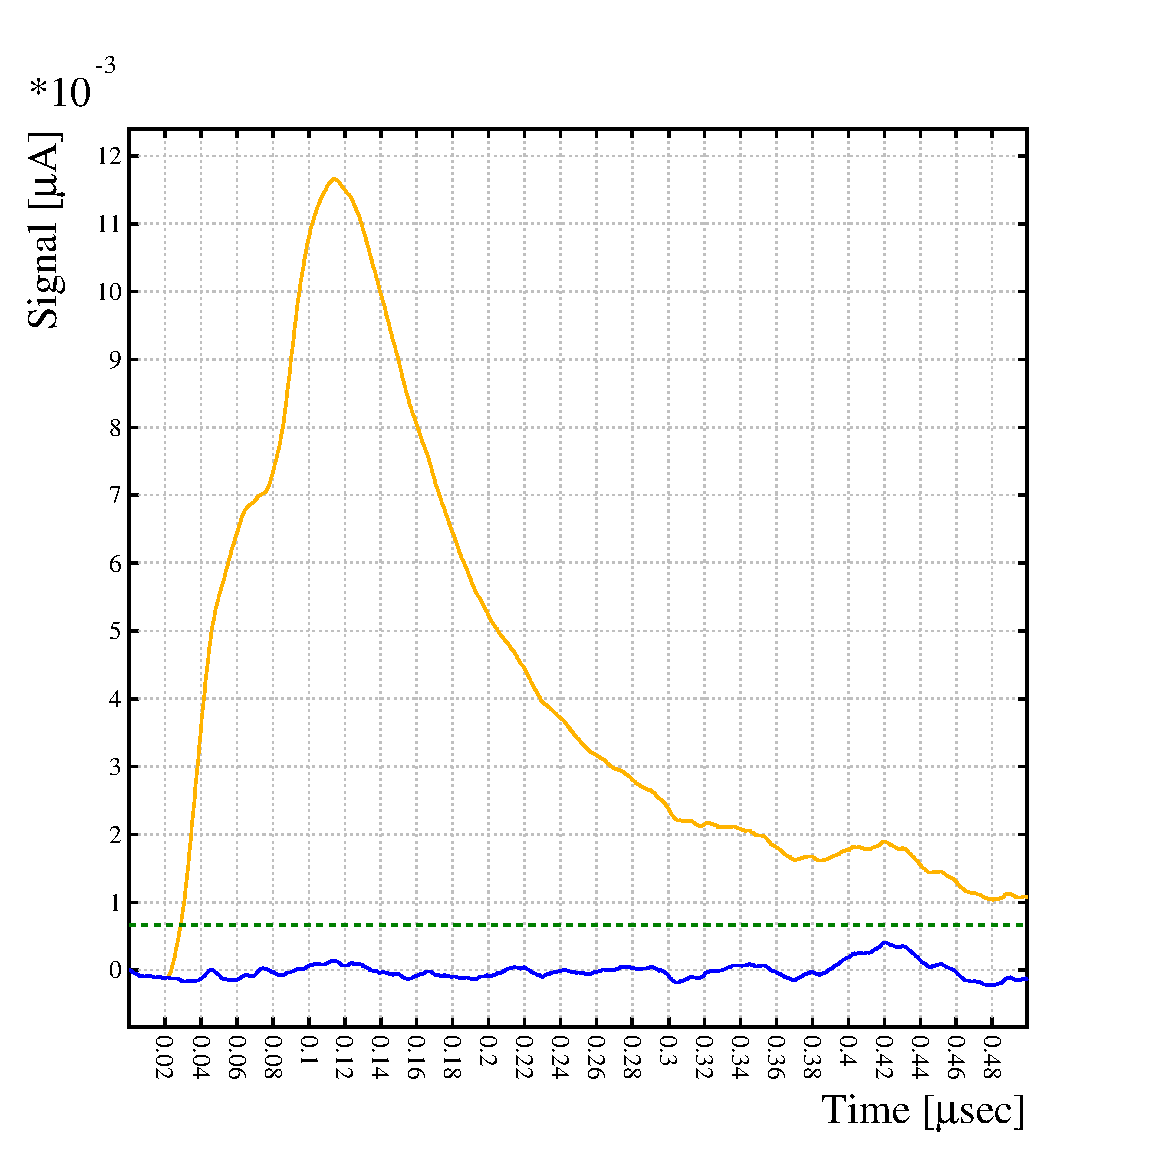
\includegraphics[width=0.7\textwidth]{signal_noise_threshold.eps}
	\caption{ Example of output signal $V(t)$ after convolution(front-end electronics) from central track(yellow line). The noise component of the same signal depicted by separate blue line. Grin dashed line is a threshold for trigering drift time and equal to $5\sigma$ of noise distribution.}
%	Приблизний сигнал(напруга) на виході з формувача зчитувальної електроніки(жовта лінія). Складова шуму позначена синьою лінією. Зелена лінія відповідає напрузі 5 середніх квадратичних відхилень розподілу шуму. (Зазнач, що по осі Y величина суть напруга, проте домножена на сталий коефіцієнт, далекий від правди $\sim \frac{1}{Gain}$)
	\label{fig:signal_example}
	\end{figure}
	
	\subsection{ STRAW efficiency}
	
	The interaction of charge particle with gas molecules nave probabilistic nature. For short distance tracks(somewhere at the tube periphery) the probability of tracks that do not produce any electron/ion pair becomes significantly high.
		
	The number of produced ionization clusters directly affects the hit efficiency profile. \cite{kozlinskiy} Smaller ionization length increase hit efficiency because of more ionization clusters per length unit are producing. In GARFIELD we can easily calculate amount of clusters per track. In fig. \ref{fig:cluster_distrib} you can see a distribution of number of clusters per central track for our STRAW tube. It mean that straw efficiency will be lower at the tube wall( see fig. \ref{}).
		
%	Взаємодія зарядженої частинки з молекулами газової суміші всередині STRAW tube має імовірнісний характер. Тож можуть виникати ситуції коли частинка, що прошиває drift tube не утворить жодного іон-електронного кластеру в об’ємі трубки. Даний ефект особливо наглядно спостерігати в областях трубки де довжина треку через об’єм трубки зовсім невеликий. Фактично це  треки, що проходять біля краю трубки.
	
	
	\begin{figure}[h!]
	\centering
	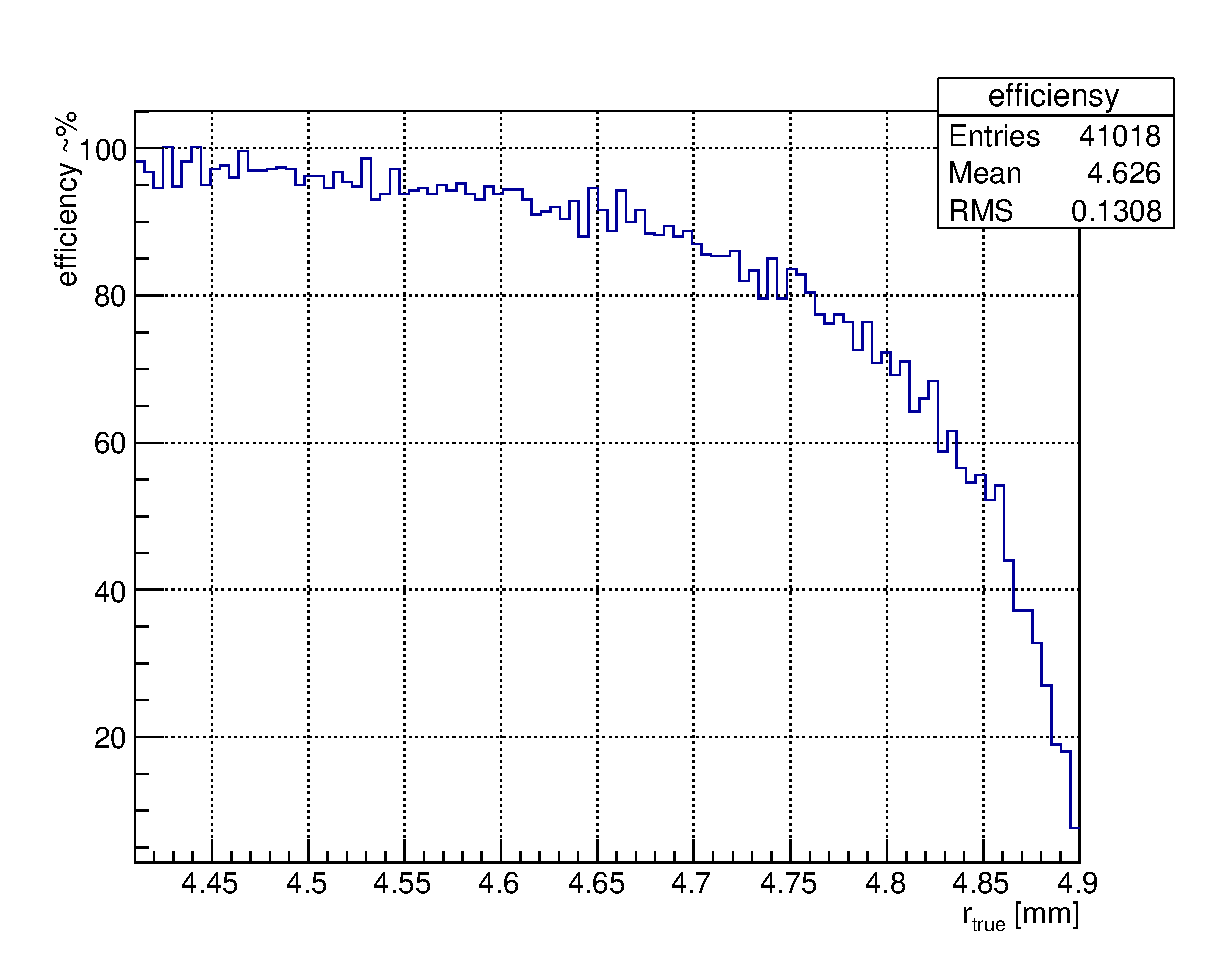
\includegraphics[width=0.9\textwidth]{periffEff}
	\label{fig:efficiency}
	\caption{ Straw tube efficiency. Result of homogeneous penetrating periphery of tube by 50k events(scaled down by factor of 5. $\dfrac{50k~events}{100 bin}  \approx 500 \dfrac{eventst}{bin}$). \textcolor{red}{NOTE: We have some wrong calculation for this plot. Especially I'm going to make new plot with 100 binning with 500 track. And as wad detected we have some mistakes in calculation. I have to replace this plot next update} }
%	Ефективність реєстрації треків в області периферії трубки від рівномірного опромінення 50 тис. треків
	\end{figure}	
	
	\begin{figure}[h!]
		\centering
		\subfloat[electrons per cluster]{
			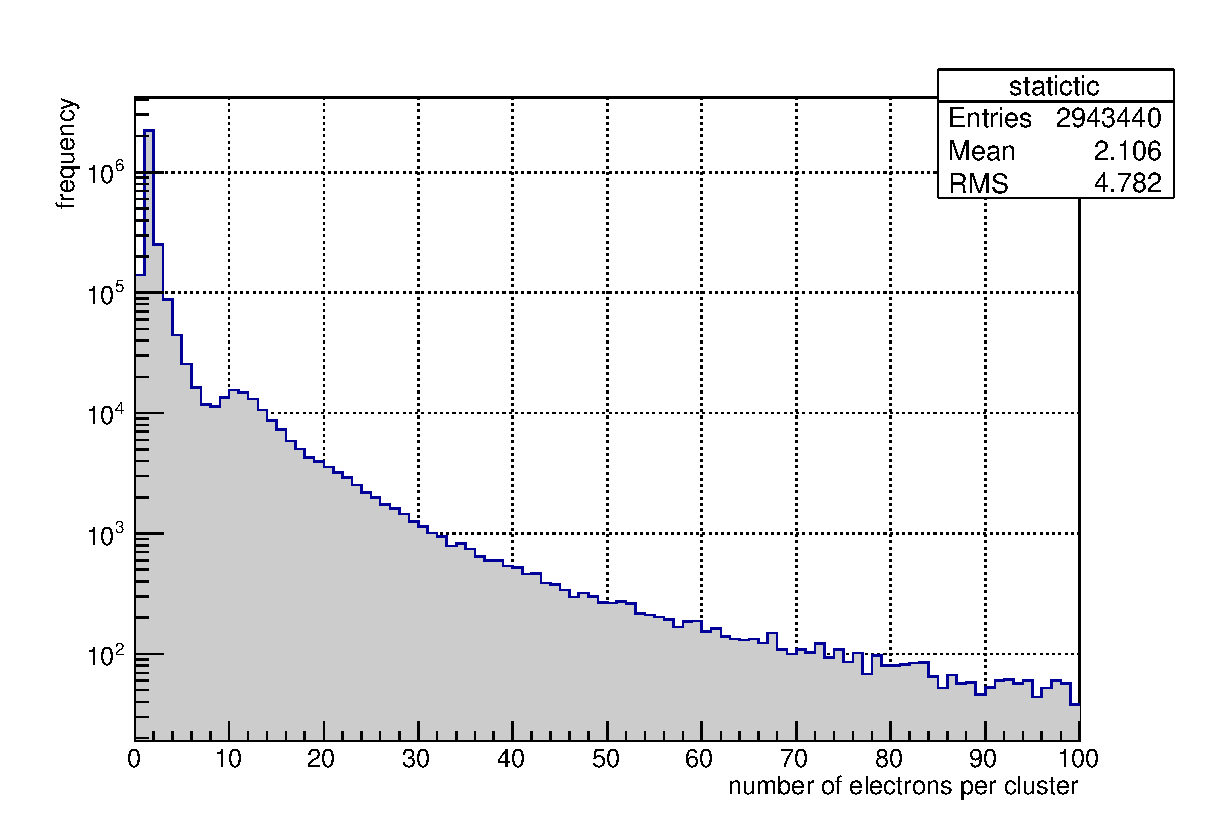
\includegraphics[width=0.45\textwidth]{el_per_cluster} 
			\label{fig:el_per_cluster} }%
		\qquad
		\subfloat[number of clusters per central track]{
			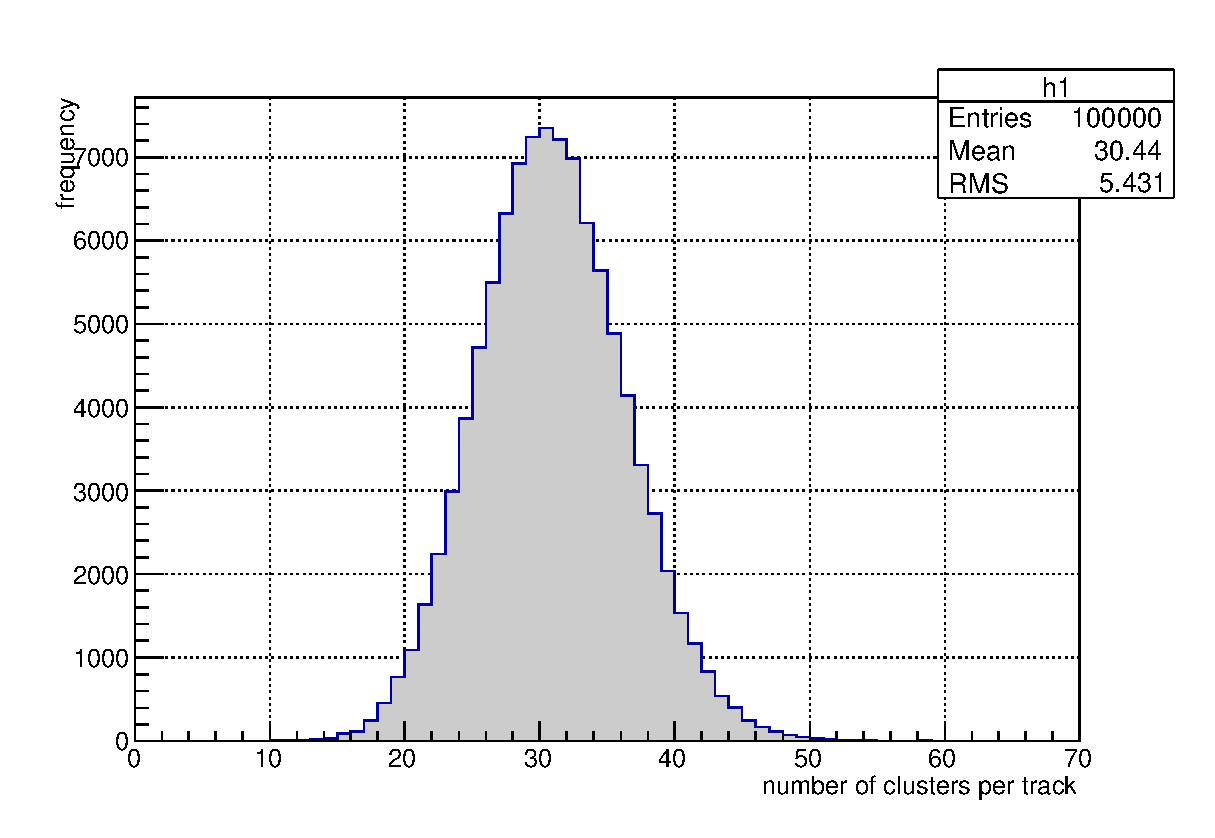
\includegraphics[width=0.45\textwidth]{cluster_distrib} 
			\label{fig:cluster_distrib} }%
		\caption{ \textcolor{red}{ There are big amount of graphs. So I'm trying to pair it. ere we can write something if needed. Some common description of (a) and (b) figures?} }
	\end{figure}
	
	From the figure \ref{fig:efficiency} we can conclude that the efficiency of tube is $100\%$ almost in whole region covered by tube except pre wall region which is quite small. Increasing the gas mixture density or increasing the tube radius for the same gas density can increase tube efficiency. Have to check this in feature studies.
	
	
%	Як видно з Рис. \ref{fig:efficiency} ефективність реєстрації сягає майже 100\% за виключенням пристінкових областей, де ефективність падає за рахунок зменшення області пробігу частинки.
	
%	Також наводимо розподіл кількості електрон-іонних пар для центрального треку(тобиш той що проходить через центр трубки) Рис. \ref{fig:n_cluster_distr}. Тож враховуючи що з частотою кластерів, порядку $\sim 3 \frac{cluster}{mm}$ можна стверджувати, що ефективність реєстрації треків у STRAW tube буде високою і близькою до 100\%, що й наглядно показано на рис. \ref{fig:efficiency}.
	
%	Hа практиці, даний показник зазвичай гірший приблизно вдвічі(на прикладі експерименту NA62 \cite{}
	 
	\section{Gain}
	
	If multiplication occurs, the increase of the number of electrons per path $ds$ is given by
	
	\begin{equation}
		dN = N \alpha ds
		\label{eq:diffGain}
	\end{equation}
	
	The coefficient $\alpha$ is determined by the excitation and ionization cross sections of the electrons that have acquired sufficient energy in the field. It also depends on the various transfer mechanism and electric field E and increases with the field because the ionization cross-section goes up from threshold as the collision energy $\varepsilon$ increases. As we can suppose the coefficient $\alpha$ is of big amount of parameters.
	
	The amplification factor $G$ on a wire(that is more interesting for us) is given by integrating (\ref{eq:diffGain}) between the point $s_{min}$ where the field is just sufficient to start the avalanche and the wire radius $a$:
	
	\begin{equation}
	G = N/N_0 = exp \int\limits_{s_{min}}^{a} \alpha(s) ds
	\end{equation}
	
	GARFIELD can provide us by amplification factor $G$ for any point of the tube(because  $G$ is coordinate dependent magnitude). The amplification factor is equal almost in whole tube space except neighbourhood near the wire because electric field  becomes significantly high only near the wire (see figs \ref{fig:elFieldCentered}, \ref{fig:elField1mmShifted}). When the wire is shifted from the center of the cube the electric field in area close to the wire is the same as in centered state. So the amplification factor $G$ is quite similar in both cases.
	
	\begin{figure}[h!] 
		\centering
		\subfloat[electric field for centered wire]{
			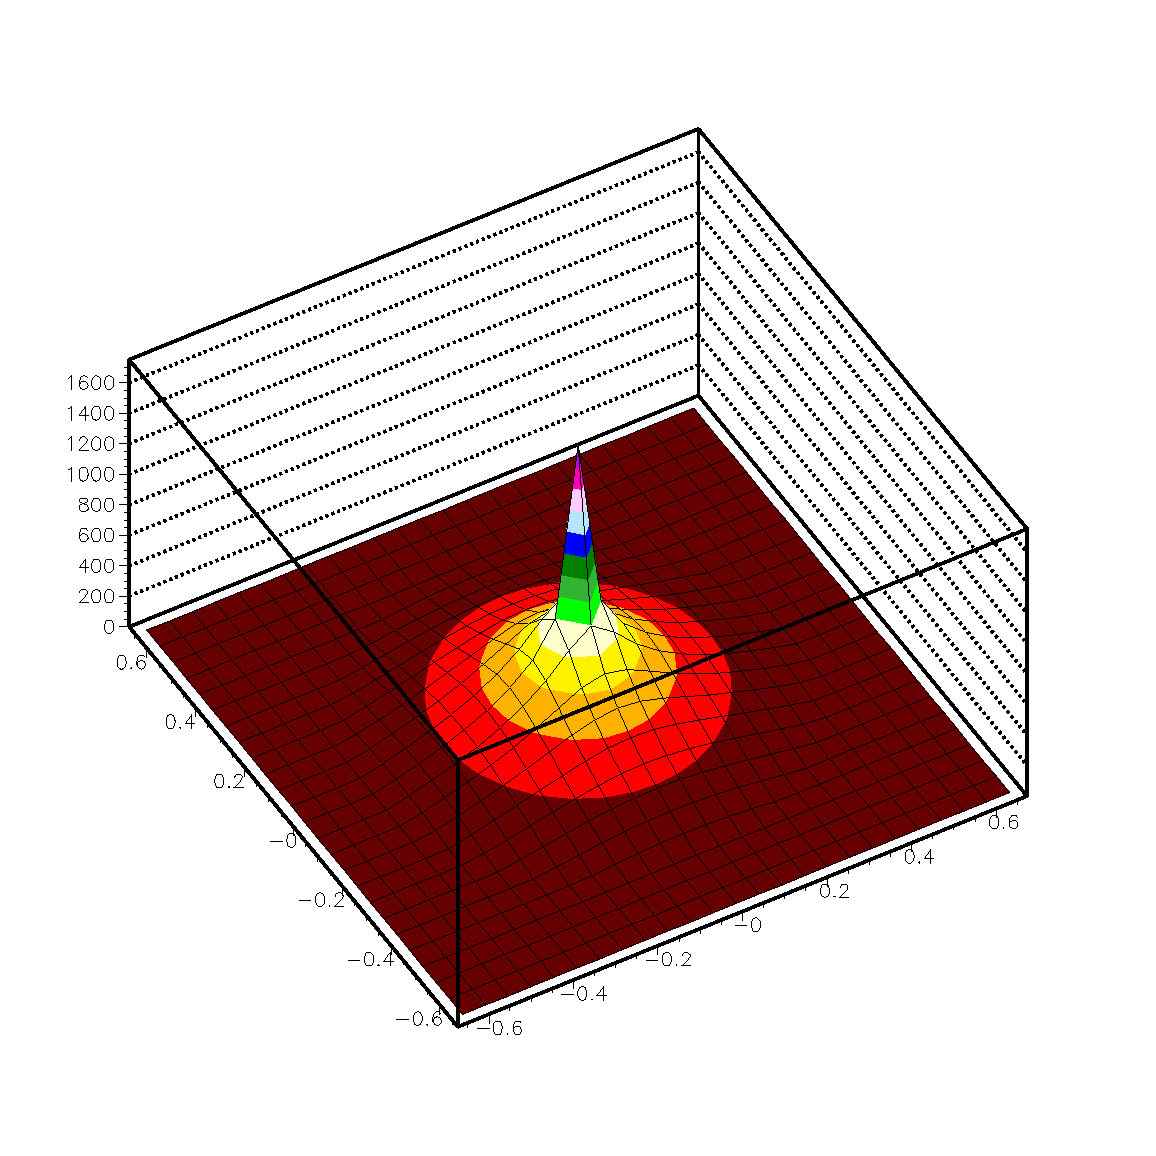
\includegraphics[width=0.45\textwidth]{fieldCentered} 
			\label{fig:elFieldCentered} }%
		\qquad
		\subfloat[electric field for $1 mm$ shifted wire]{
			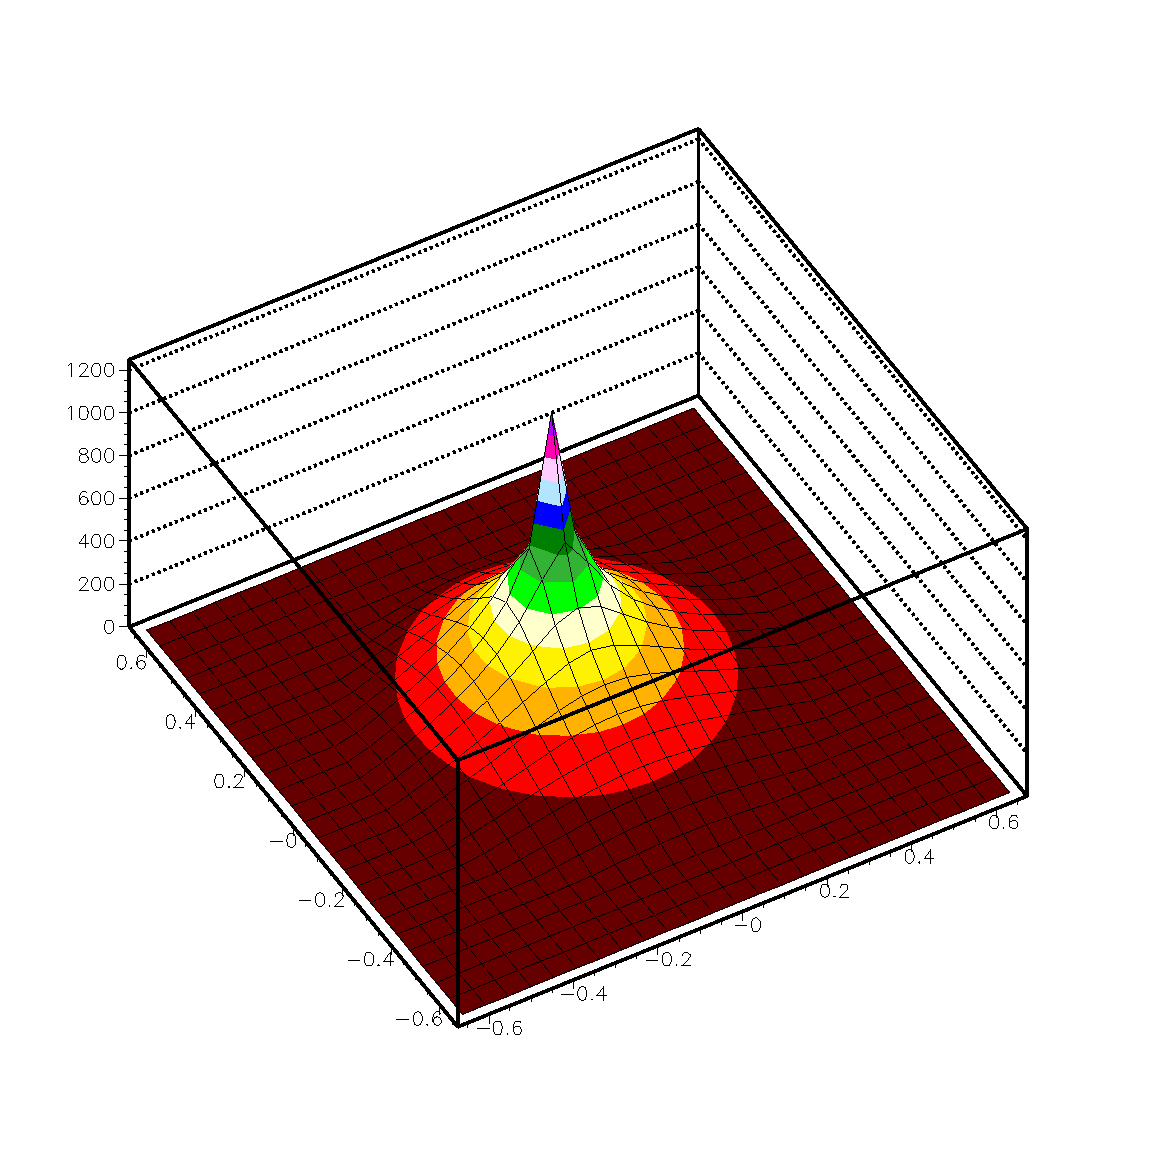
\includegraphics[width=0.45\textwidth]{field_10Sag}
			\label{fig:elField1mmShifted} }%
		\caption{Electric field intensity map for different wire position in the cube calculated in GARFIELD software. Conditions for those plots are described in table \ref{table:straw_par} }
	\end{figure}
	
	Implementation of gain value calculation is not so reliable in GARFIELD(especially fortran version). So we can reach better results using Garfield++ (which is newer and take into consideration more effects).
	
%	На базі оцінки форми сигналу та амплітуди вихідного струму каналу STRAW трубки проектується відповідна front-end електроніка. Коефіцієнт газового підсилення залежить від складових газової суміші, тиску, температури і поля в якому рухаються електрони/іони і розвиваються електрон-іонні лавини.
	
%	Власне імплементація скрипту для розрахунку коефіцієнта підсилення у програмному пакеті Garfield вимагає від нас знання параметрів ефекту пеннінга для \cite{} для розглядуваної газової суміші.
	
%	Приведемо графік залежності коефіцієнту підсилення сигналу для суміші газу зазначеної в таблиці \ref{table:straw_par} від напруги на дроті STRAW трубки.

	On the Fig.~\ref{fig:gain-voltage-dendence} you can see that the gain $G(V)$ have precisely exponential dependence. This is frankly does not inspire confidence. The difference can be up to 100\% (us Rob Veenhof\cite{garfield} said).
	
%	Як видно, з Рис.~\ref{gain_trought_voltage} він носить точно експоненціальний характер, що, чесно кажучи не викликає особливої довіри, хоча напевне є з певною точністю справедливим. 
	
%	Попри це механізм розрахунку коефіцієнту підсилення в програмному пакеті Garfield реалізований недостатньо якісно, в тому сенсі, що на момент написання пакету Garfield (fortran версії) процес газового підсилення був вивчений не достатньо добре. Використання програмного пакету Garfield++ може вирішити цю проблему, так як написаний пізніше і дозволяє отримати значно точніші і достовірніші дані. Зі слів Rob Veenhof точність може різнитися в РАЗИ.
	
%	Дана перспектива може бути виконана в майбутньому як частина даної дипломної роботи.
	
%	Наразі маємо можливість побудувати залежність залежності коефіцієнту газового підсилення електромагнітної лавини в газі(gas gain). Для оцінки коефіцієнту підсилення 
	
	\begin{figure}[h]
	\centering
	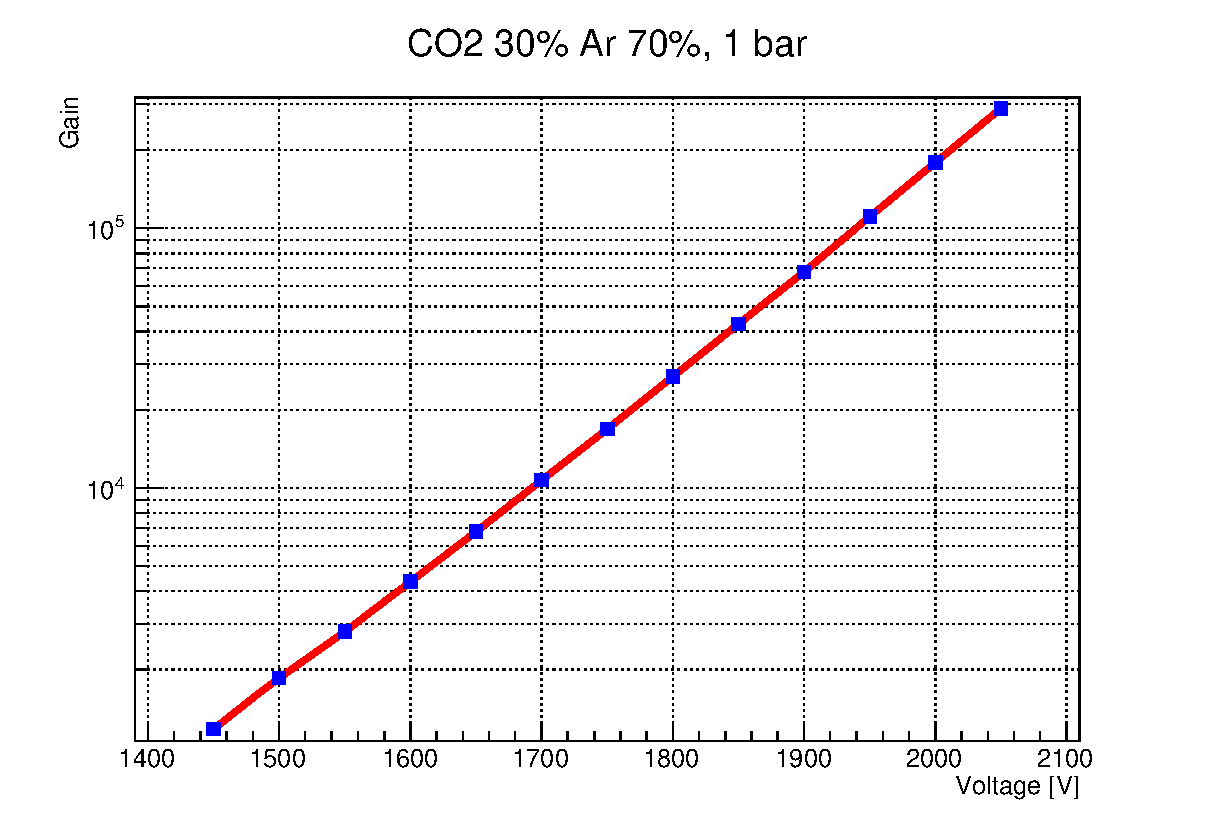
\includegraphics[width=\textwidth]{gain_1450_2050V}
	\label{fig:gain-voltage-dendence}	
	\caption{Dependence of the gain of the voltage applied to the wire. The rest of STRAW tube settings you can find in table \ref{table:straw_par}}
%	Графік залежності коефіцієнту підсилення сигналу в трубці(gain) в залежності від прикладеної до дроту напруги. Параметри системи описані в таблиці №\ref{table:straw_par}}
	\end{figure}
	
	\section{ Wire sagging}
	Easy to predict that the shifting of the wire invoke distorting an electric field and drift path for electrons/ions inside the tube(see fig.\ref{fig:electron_ion_track} and fig.\ref{fig:electron_ion_track_sag}). So the rt-relation for track reconstruction directly depend on the wire position in the tube. rt-relation lose it's previous symmetry(see next sections). 
	
	\begin{figure}[h!]
		\centering
		\subfloat[wire in the center of the tube]{
			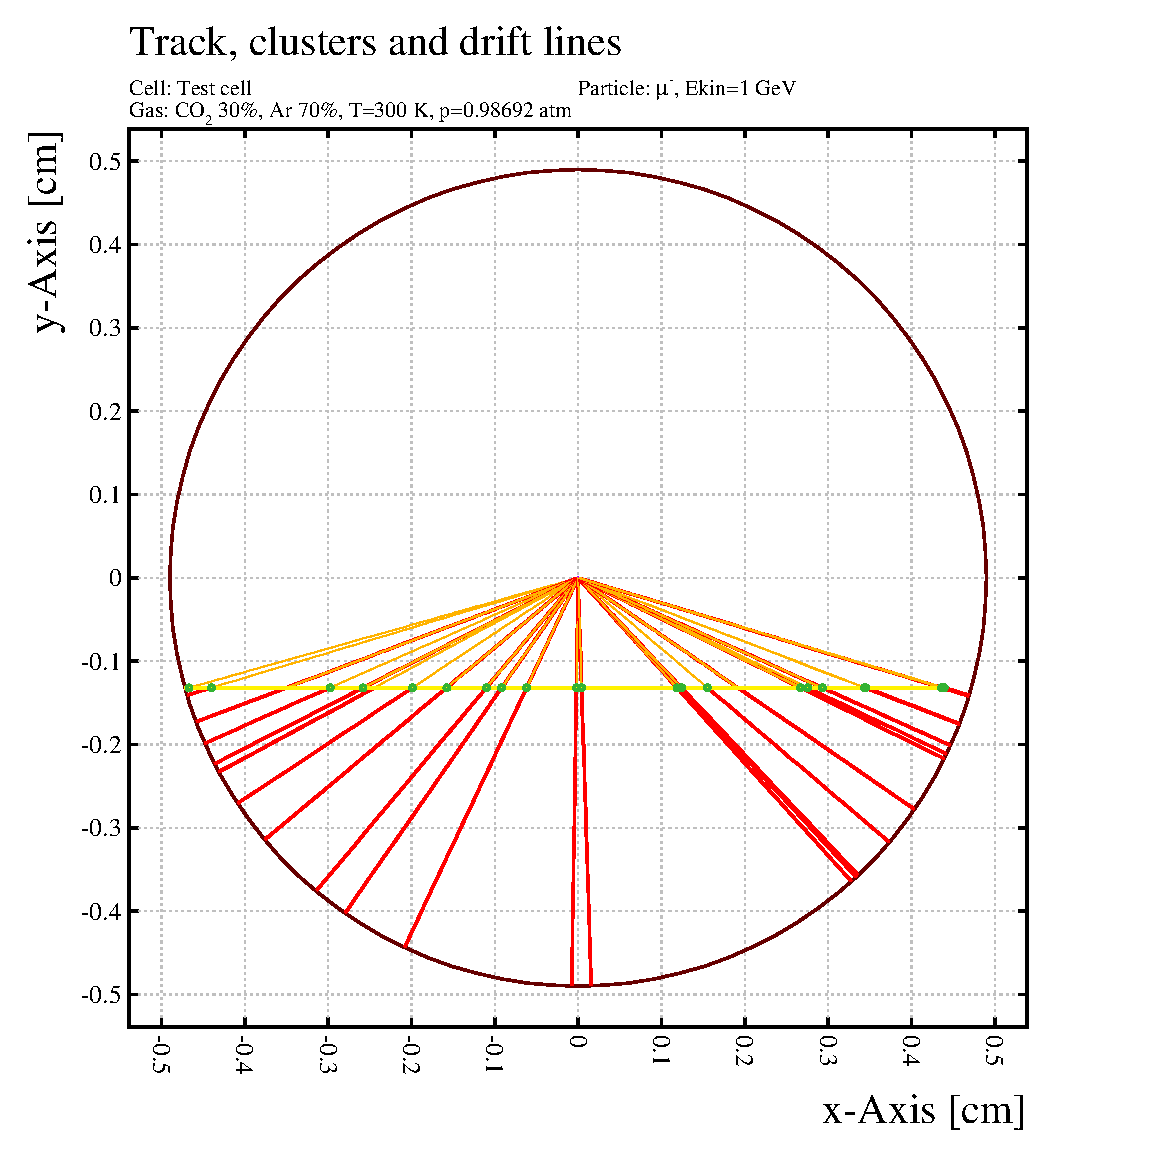
\includegraphics[width=0.45\textwidth]{tracksAndClusters00Sag.eps} 
			\label{fig:electron_ion_track} }%
		\qquad
		\subfloat[sagging $1.5 mm$]{
			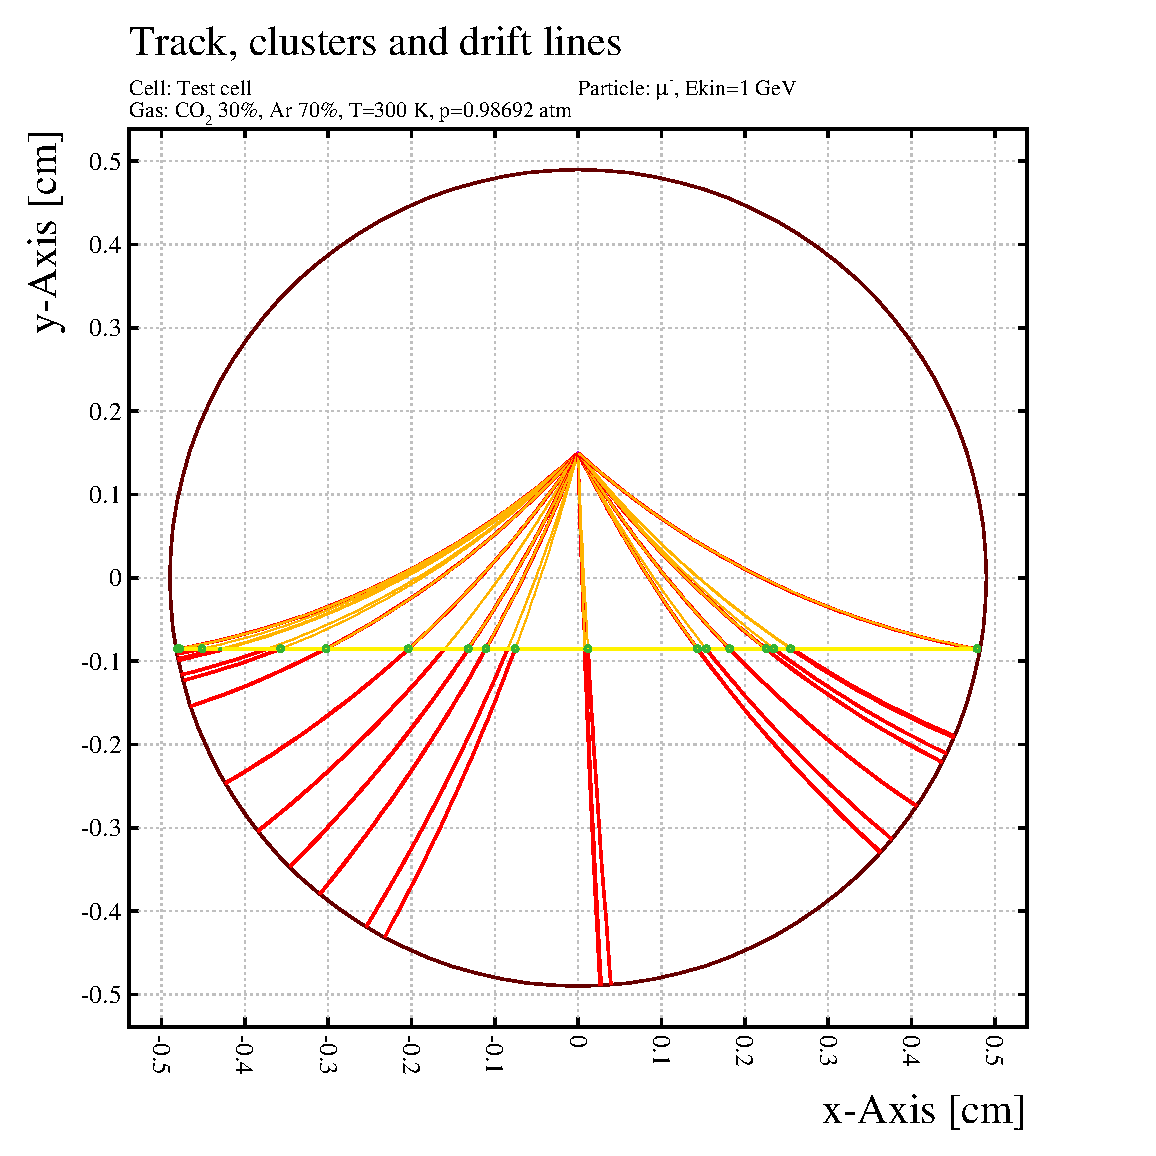
\includegraphics[width=0.45\textwidth]{tracksAndClusters15Sag.eps} 
			\label{fig:electron_ion_track_sag} }%
		\caption{ An example of tracks from the on the tube for different position of the wire from GARFIELD simulations. Initial clusters marker by green. Drift lines for electrons marked by yellow, ions -- red lines.}
%		Приклад траекторії руху електронів та іонів в дрейфовій трубці в результаті проходження зарядженої частинки в горизонтальному напрямку(перпендикулярно до напрямку провисання трубки в площині поперечного перерізу дрейфової трубки}			
	\end{figure}
	
	The direction of sagging is unpredictable when the wire is centered and the straw has vertical orientation. Impact of gravitation field into the wire does not make any effect in this state. But we can avoid this ambiguity by setting straws horizontally. This condition is necessary to make track reconstruction possible.
	
	We estimate significant wire sagging(by comparison to the tube radius) because of wire attracts to the tube under affecting of gravitation and electric field force.
	
	
%	Під дією сильного електричного поля дріт(анод $V_{wire}\cong1750 V$) притягується до стінок трубки (катод $V_{tube}=0V$) і так зване провисання досягає значних розмірів $\sim1.5mm$ при радіусі трубки всього $4.9 mm$.
	
	You can see a profile of wire sagging of $5m$ length wire in $1cm$ diameter straw tube and 1750V voltage on the fig.\ref{fig:sagProfile} calculated in GARFIELD software \cite{garfield}.
	
	\begin{figure}[h!]
	\centering
	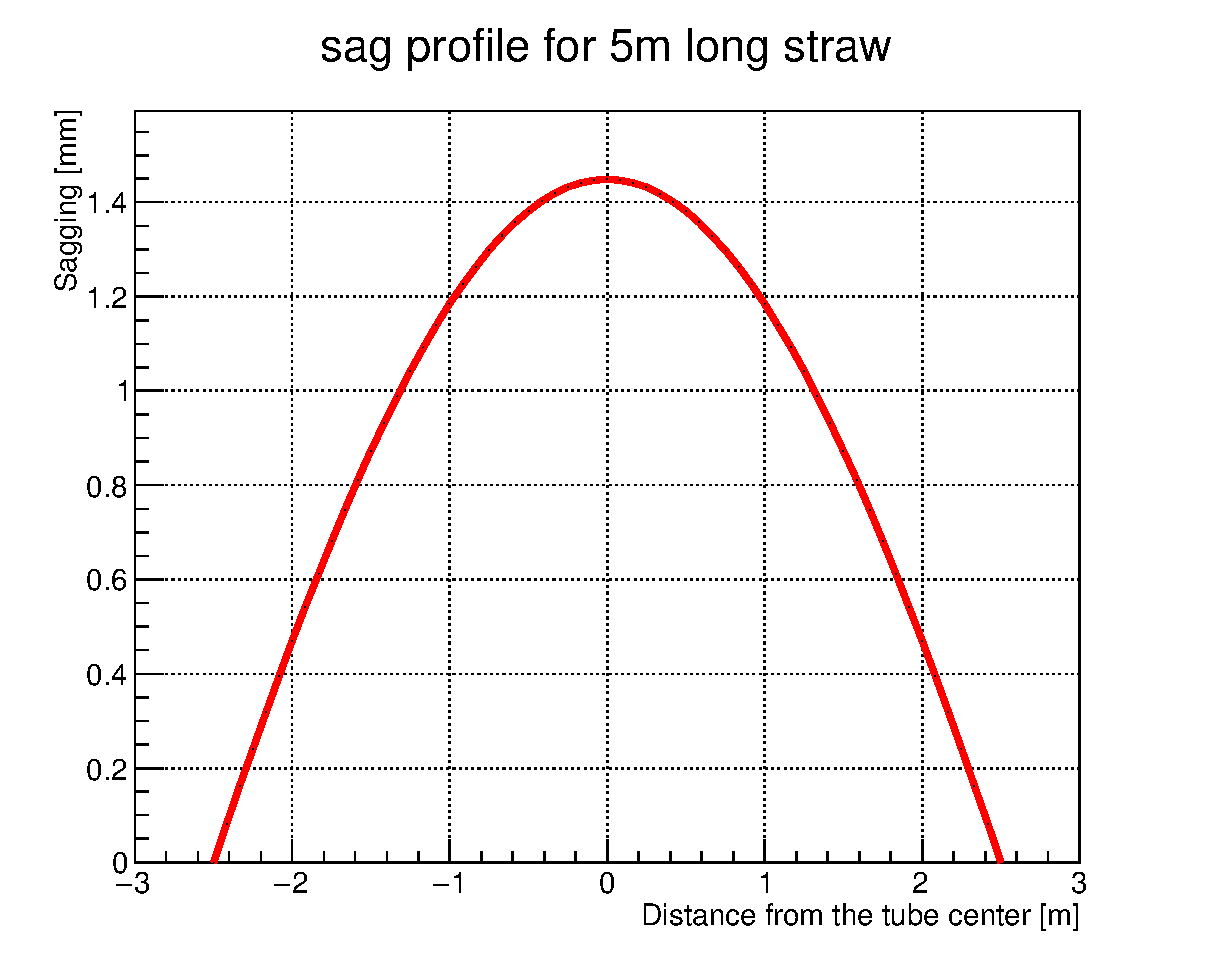
\includegraphics[width=0.7\textwidth]{sagProfileFit.eps}
	\caption{Wire sag profile under electric and gravitation field calculated in GARFIELD. All options for this straw system are described in table~\ref{table:straw_par}.}
	%Профіль провисання проводу в дрейфовій трубці довжиною 5 метрів під дією електричного та гравітаційного полів розрaхований у програмному пакеті Garfield
	\label{fig:sagProfile}
	\end{figure}	
		
	The calibration of STRAW tube with sagged wire is more difficult by comparison to the mode without sagging. 
	
	Variation of wire tension, wire radius should be taken into account as high affect factor for sag value.
	
%	Це ускладнює роботу з дрейфовими трубками, так як в залежності від зміщення трубки від центрального положення змінюється і час дрейфу. Це ускладнює процес реконструкції треків, і вимагає додаткових кроків в процесі реконструкції треків. При чому потрібно зважати на той обсяг інформації який ми можемо витягти з дрейової трубки в робочому стані. Адже не всі методи зостосовні до калібровки трубки в лабораторних умовах можуть бути виконані на практиці при в зібраному детекторі.

%	Одним із головних припущень в даній задачі є вибір конфігурації трубок. Припустимо, що трубка є відносно ідеальна: не прогинається під дією гравітації та без викривлень в результаті дефектів при виробництві чи процесі встановленні на робоче місце, або ж якихось інших факторів). Коли трубка знаходиться у вертикальному положенні(тобо у стані, коли гравітаційне поле не впливає на початкове позиціонування дроту в трубці) напрям провисання дроту передбачити неможливо - він повністю залежить від дефектів трубки при збірці та позиціонуванні дроту при фіксації на торцях, якщо всі всі інші поля відсутні.
			
%	Проте в горизонтальному положенні трубок гравітаційного поля має бути достатньо, щоб задати напрям провисання трубок строго по напрямку гравітаційного поля $\vec{g}$. Таким чином неоднозначність конфігурації трубки зникає.
	 
	
	
	\section{ Sag estimation}
	
	Очікується, що для кожному окремому положенню дроту в трубці (зміщення від центрального положення) буде відповідати своя TR-залежність. Тож першочерговим завданням є визначити зміщення дроту в  трубці від центрального положення.
	
	Як логічно припустити з Рис. \ref{fig:t_r_distr_00} та \ref{fig:tr_distr_15} розподіл часу дрейфу  для випадків з різним значенням зміщення дроту буде також різнитися Рис. \ref{fig:DrftTimeDistr_00_09_comp}. На прикладі порівнянн  двох діаграм видна сходинко-подібна природа.
	Отже з цих розподілів легко можна отримати значення відхилення дроту в даному місці трубки.
	
	\begin{figure}[h]
	\centering
	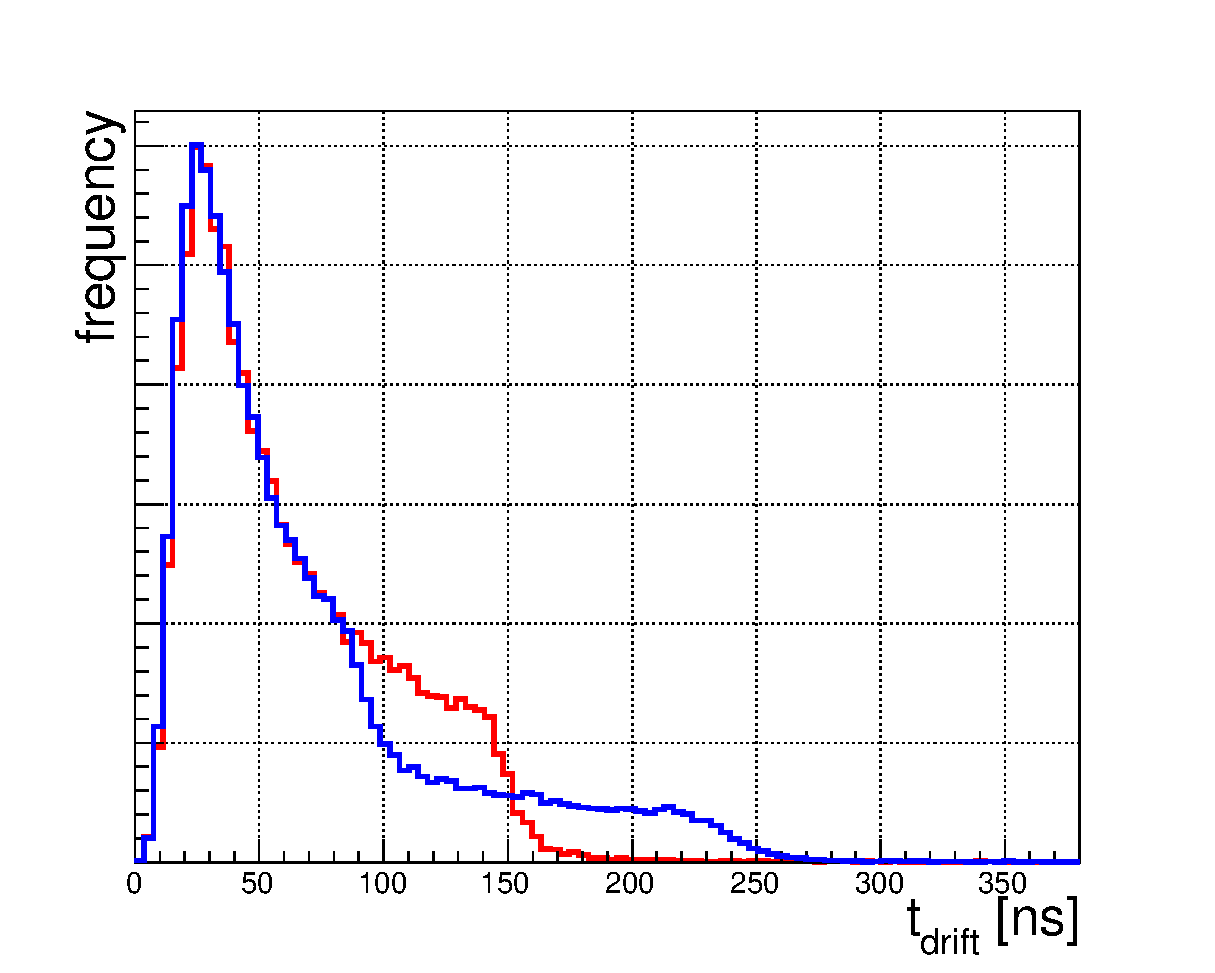
\includegraphics[width=0.8\textwidth]{00_09_driftTimeDistr}
	\label{fig:DrftTimeDistr_00_09_comp}
	\caption{Drift time distribution for a homogeneous irradi-
ation with a centered wire (red) and for a wire offset of 0.9 mm (blue).}
	\end{figure}
	
	Описані вище розподіли часу дрейфу вказані на рис. \ref{fig:DrftTimeDistr_00_09_comp} виконані в середовищі Garfield для константного положення дроту. Нажаль Garfield не дозволяє робити робити симуляції для  профілю дроту.

	Першим кроком для знаходження положення дроту з діаграм знайдемо вигляд розподілів для кожного можливого значення положення дроту в трубці. В нашому випадку було виконано симуляції для отримання діаграм в різних положеннях в діапазоні від $0$ до $1.5 mm$.

	Наступним кроком ми маємо привести у відповідність конкретний розподіл з координатою дроту для калібровки. На практиці це пропонується здійснити за допомогою оптичного просвічування трубки.
	
	На експерименті будемо визначати профіль трубки з порівняння профілю даного вимірювання з виміряними раніше "калібровочними" серіями вимірів.
	
	Робиться це настпним чином:
	\begin{enumerate}
		\item кожна діаграма нормується і рахується $\chi^2$ попарно з кожною з core діаграм. 
		\item для отриманих значень $\chi^2$ будуємо графік, де по осі Х відкладається положення дроту.
		\item Мінімум даної залежності допоможе знайти core діаграму найближчу до вимірюваної. Адже такі діаграми будуть найбіьш схожими (Рис. \ref{fig:chi2for07})
	\end{enumerate}
	
	\begin{figure}
	\centering
	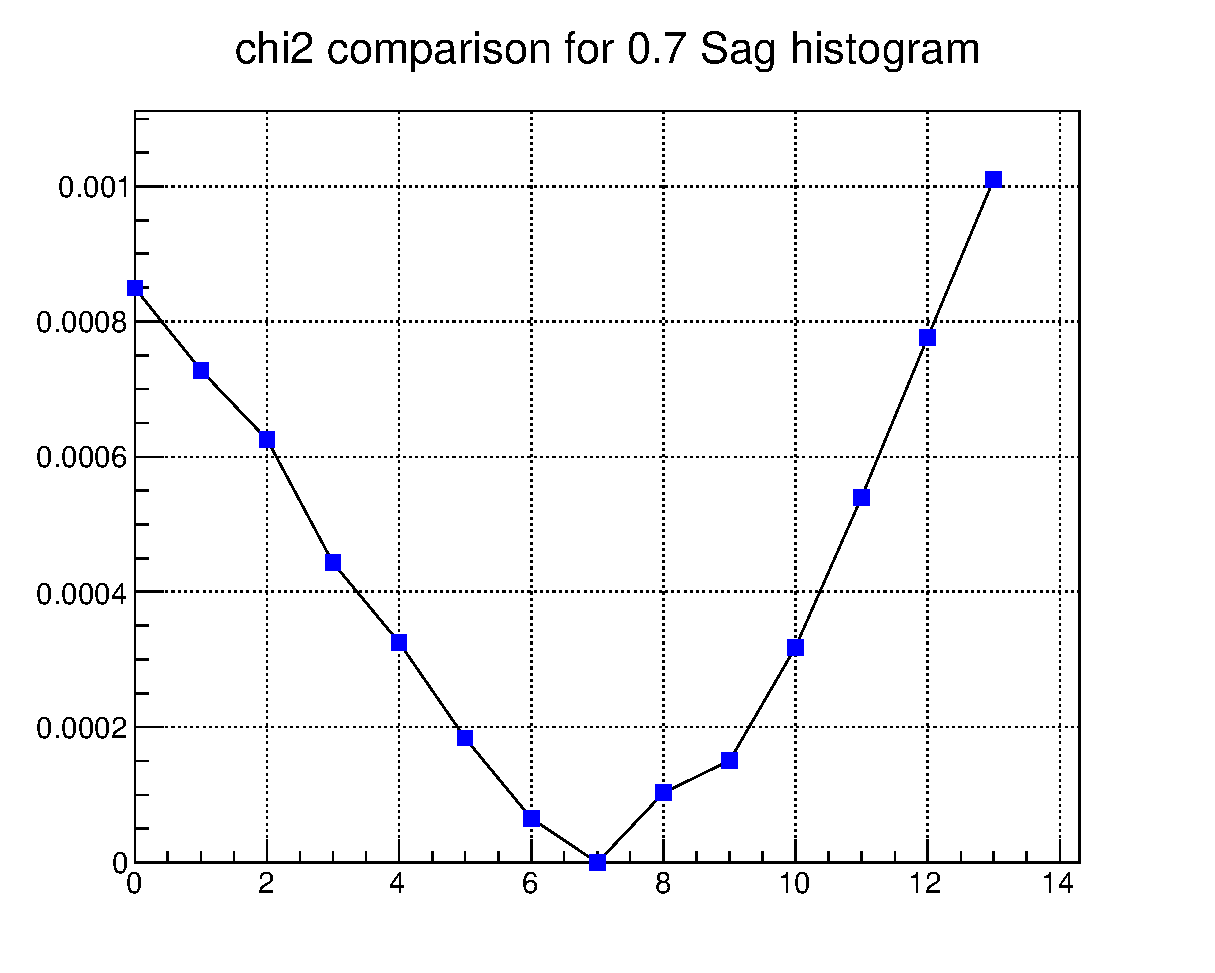
\includegraphics[width=0.8\textwidth]{chi2_07}
	\caption{ Порівняння $\chi^2$ для core діаграми $0.7 mm$ з усіма іншими core діаграмами в діапазоні $0\dots 1.5 mm$}
	\label{fig:chi2for07}	
	\end{figure}
	
	Точність даного методу може бути достатньо великою. Для діаграм статистикою 5 тисяч подій розподіл визначення визначення положення дроту зображено на Рис. \ref{fig:chi_063_5k}
	
	На експерименті вказані вище розподіли отримати не важко. Єдине що потрібно набирати статистику лише для фіклованого положення дроту, а значить необхідно проводити експозицію секційно -- не по всій довжині трубки а лише на відповідних ділянках, таких щоб значення відхилення дроту на них не відрізнялося більше необхідної точності.
	
	Нехай бажана точністю визначеня положення дроту $50 \mu$. Розділивши весь дріт на ділянки маємо, що центральний сектор буде найбільшим і має довжину $0.8 m$. Це при значенні максимального просідання дроту $1.5 mm$.
	
	
	\begin{figure}[h]
	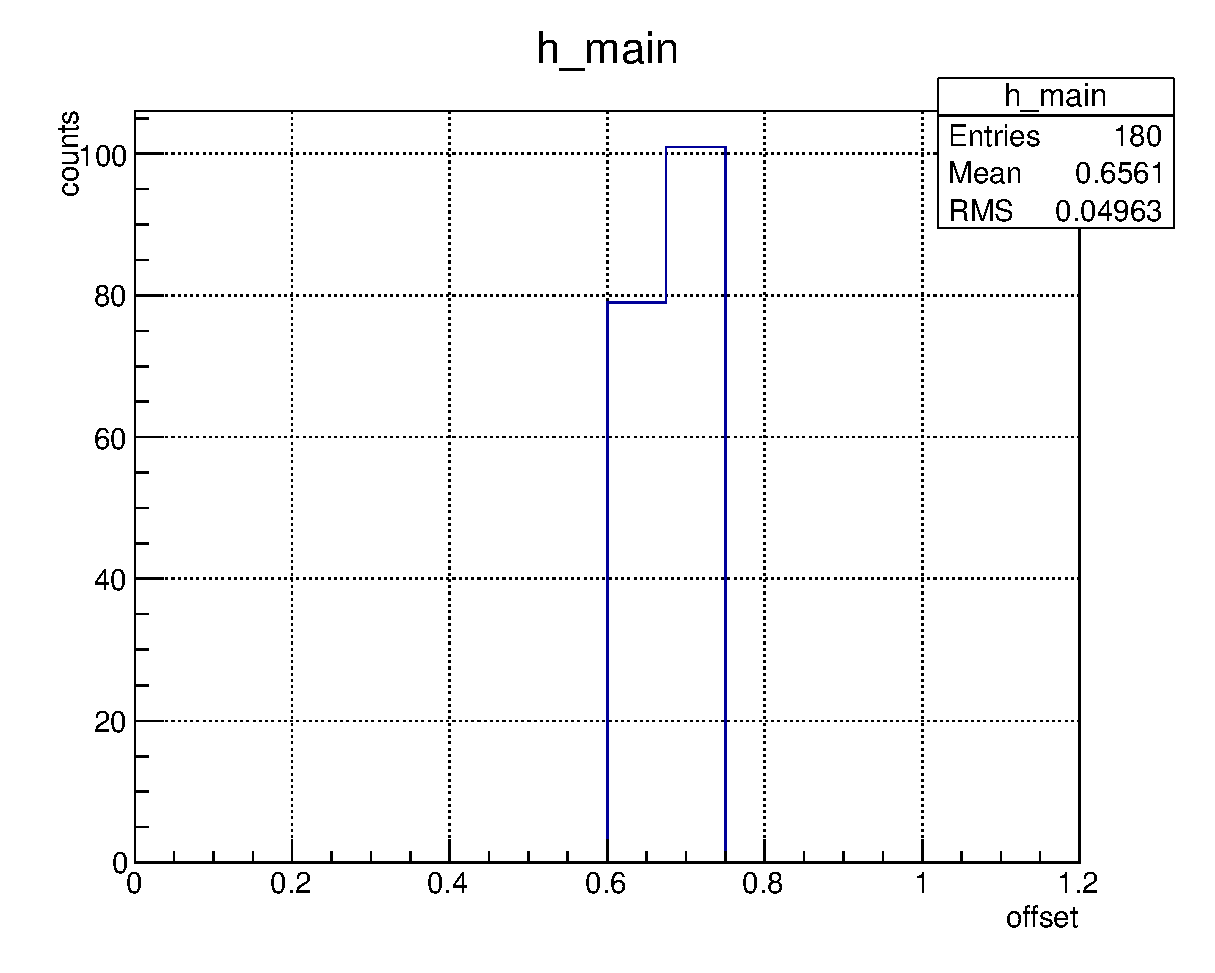
\includegraphics[width=0.8\textwidth]{chi_063_5k.eps}
	\centering
	\caption{ Bias estimation distribution for 5k data. 50k events for core template histograms. True bias is 0.063 mm. 1 bin = 0.1 mm. } 
	\label{fig:chi_063_5k}
	\end{figure}
	
	
	\section{Track reconstruction}
	
	 The time between the track hit time stamp and the signal at the wire at the wire is a measure for {\it drift time} of these electrons. The relation between the   {\it drift time} and  the distance from the track to the center of the tube(wire while no sag for centered wire) is called {\it drift time - distance relation} or {\it rt-relation}.
	
	The drift time $t$ is a function of track position relative to the wire(so it mean the track position) and electric field along the drift trajectory.
	
	Assumed that the working  position  for straws will be parallel to the particle bunch, and particle speed acceptance will not be significantly big. So tracks will be collinear each other for every separate unit STRAW tube.
	
	Summing the above mentioned we have one dimension task -- reconstruct tracks on vertical axis\footnote{An example of single track reconstruction which explaining the approximate procedure of reconstruction you can see in Fig.\ref{fig:track_reconstruction}}
	(see example outcome rt-distribution $t = t(r,s=0)$ in Fig.\ref{fig:t_r_distr_00} ) even the wire sagging. Sagging will be always down thanks to gravitation force $\vec{g}$.
	
	\begin{figure}[h]
	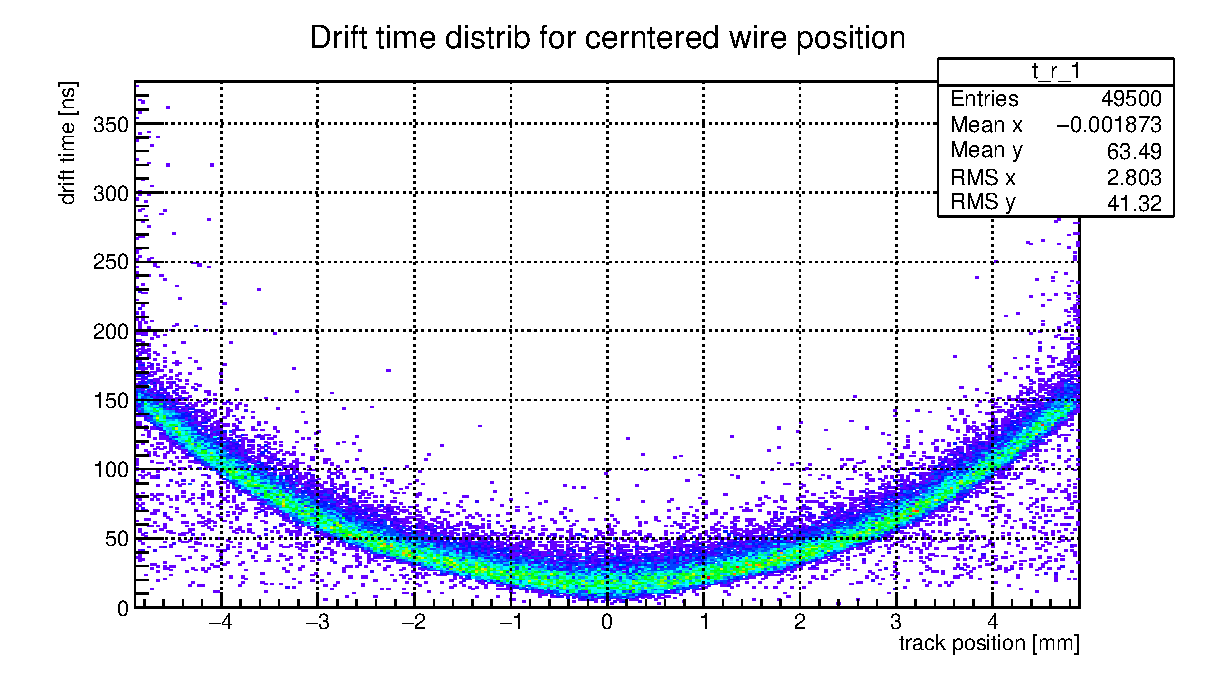
\includegraphics[width=0.8\textwidth]{t_r_distr_00.eps}
	\centering
	\caption{ Distribution of drift time $t_{drift}$ as function of track position $r_{track}$ relatively to the tube center} 
	\label{fig:t_r_distr_00}
	\end{figure}
		
	The rt-relation is differ along the tube because different wire position $s$. We thus have for the drift time 
	\begin{equation}
	t = t(r_{track},s)
	\end{equation}
	
	\subsection{ Double ambiguity in track reconstruction}
	Usually the outcome of first step reconstruction is two position.
	
	
%	Після проходження зарядженої чатинки через об’єм дрейфової трубки вздовж треку виникають електрон іонні кластери, які під дією сильного електричного поля починають дрейфувати до відповідних електродів викликаючи струм у електричному колі дрейфової трубки. Слідом, ненульовий струм кола дрейфової трубки відповідає руху зарядів в о’бємі трубки. Час дрейфу найближчих до аноду електронів містить інформацію про положення треку в трубці, тож по моменту часу переднього фронту сигналу можна відновити положення треку, а точніше радіус кола дотичного до треку і паралельного трубці. Надалі будемо позначати {\it часом дрейфу} проміжок часу від моменту появи треку до перевищення вихідним сигналом певного порогового значення(зелена штрихована лінія на Рис. \ref{fig:signal_example}).
	
	\subsection{Джерела похибок}
	
	\begin{itemize}
		\item Природна складова похибки визвана розподілом кластерів іонізованих атомів вздовж треку MIP-частинки.\par
		\item Похибка пов’язана безпосереньо з дрейфом електронів та йонів в трубці. Залежить від параметрів електричного поля та складової газу в трубці.
		\item Похибка пов’язана з ефектами поширення заряду від електромагнітної лавини в дроті.
		\item Фактори електроніки -- функція відгуку електроніки.
	\end{itemize}
	
	\subsection{Геренерація шуму}
	Шум -- штука непердбачувана, і дуже залежить від технологічного процесу виготовлення складових елементів детекторної систреми. Шум в кінцевому результаті дуже впливає на якість вихідних даних детектора: його ефективність реєстрації, роздільну здатність.
	
	Шум зараз особливо важко оцінити, так як робочих екземплярів дрейфових трубок ще нема, і front-end електроніки в тому ж числі нема.
	
	Тож задамо шум з огляду детекторних установок подібного типу.
	
	Програмний пакет Garfield дозволяє задати значення струму шуму через імовірнісну функцію розподілу. Підберемо такий розподіл струму, щоб вихідна напруга перед дискримінатором (умовно кінцева напруга) була розподілена за гаусом 
	$P_{\mu,\sigma}(x) = Ae^{\frac{-(x-\mu)^2}{2\sigma^2}}$ 
	з середнім розподілу $\mu=0$ та з середнім квадратичним розподілом рівним сигналу від дрейфу 2000 електронів $ \sigma = 2000e$ -- так званий electric noise charge (ENC). Приклад сигналу шуму зображено на Pис. \ref{fig:signal_example}
	
	Дане питання одне із слабких місць даної симуляції і в майбутньому будуть проводитися зміни. Тож дана частина є нічим іншим як костиль.

	
	\section{Знаходження параметрів калібровочної кривої}
	
	Калібровочною кривою в даному випадку будемо називати функцію, яка є оптимально відповідність між часом дрейфу та нійблільш імовірним положенням треку(наприклад радіус кола, дотичного до лінії треку частинки концентричного до поперечного профілю трубки).\\
		
	\subsection{Випадок центрованого дроту}
	Хоча, я відчуваю "симетричний випадок" і не ввійде в мою роботу і до розгляду буде одразу представлений загальний випадок знаходження калібровочної кривої я всеодно виділю окремий розділ. Частина з нього точно буде присутня у фінальній версії диплому(як мінімум рисунки).
	
	До початку розглянемо випадок, коли дріт трубки розташований строго по центру і можна застосувати спрощену процедуру для побудови RT - залежності. Частинки, що проходять крізь дрейфову трубку на однаковій відстані мають викликати сигнал з однаковими часовими характеристиками зростаючого фронту. 
	
	Знаючи час дрейфу можемо відновити дотичне до треку коло. Якщо ж напрямок поширення частинки відомий то кількість можливих положень частинки зводиться до двох. На експерименті очікується, що дрейфові трубки будуть розташовані в площині перпендикулярній до напрямку пучка. Тож залишається серед двох дзеркальних до дроту треків вибрати один. Ця задача легко вирішується вже в процесі комбінаторики відновлення треку по хітах.
	
	

	
	
	
	Калібровочну криву будемо знаходити з апроксимації розподілу $t_{drift}(r)$ Рис.\ref{fig:t_r_distr_00}.
	
	Instead of using the average value of the drift time residuals, a fit to the distribution of unbiased drift time residuals is performed in a narrow range around the peak. This allows to reduce the contribution of incorrectly assigned hits

	Для ясності опишемо дану процедуру поетапно
	\begin{enumerate}
	\item Оскільки TR розподіл симетричний відносно $r_{track} =0$ Рис.~\ref{fig:t_r_distr_00}, то для підвищення статистики будемо аналізувати їх "суму".
	\item з TR розподілу рис.\ref{fig:t_r_distr_00} будуємо структурну діаграму шляхом розбиття даних на секції вздовж $r_{track}$ (ось Х) і знаходимо середнє для таких вибірок.
	\item як видно з рис.\ref{fig:t_r_distr_00} в симуляціях є досить багато шуму - точки поза головним "стержнем" розподілу. Тому для більш точних результатів в побудові RT залежності цього шуму слід позбавитися. Як варіант пропоную наступний критерій: вважати шумами всі точки, які знаходяться на відстані більше $2 \sigma $ від середнього вибірки для кожної із секцій від першої ітерації.
	\item для "відфільтрованих" даних повторюємо пункт №2;
	\item Апроксимуємо точки середнього з вибірок функцією (\ref{eq:fit_tr})
	\begin{equation}
		y = e^{a_0 +a_1x}
		\label{eq:fit_tr}
	\end{equation}
	\item Знаходимо RT відношення як оберенену до (\ref{eq:fit_tr})  функцію. Результат зображено червоною лінією на рис. \ref{fig:calibration_00}
	\end{enumerate}
	
	
	В даному випадку калібровочною кривою буде однозначна відповідність між часом дрейфу і радіусом дотичного кола.
	
	Для знаходження кривої $r(t)$ складемо дві гілки розподілу Рис. \ref{fig:t_r_distr_00} (праворуч і ліворуч нуля),	
	 інвертуємо розподіл $t_{drift}(r_{track}) \longrightarrow r_{track}(t_{drift})$ і виконаємо підгонку розподілу функцією виду (\ref{eq:calibration_func}).
	
	\begin{equation}
		\label{eq:calibration_func}
		r(t) = a_1 log(t) + a_2
	\end{equation}
	
	\begin{figure}[h]
	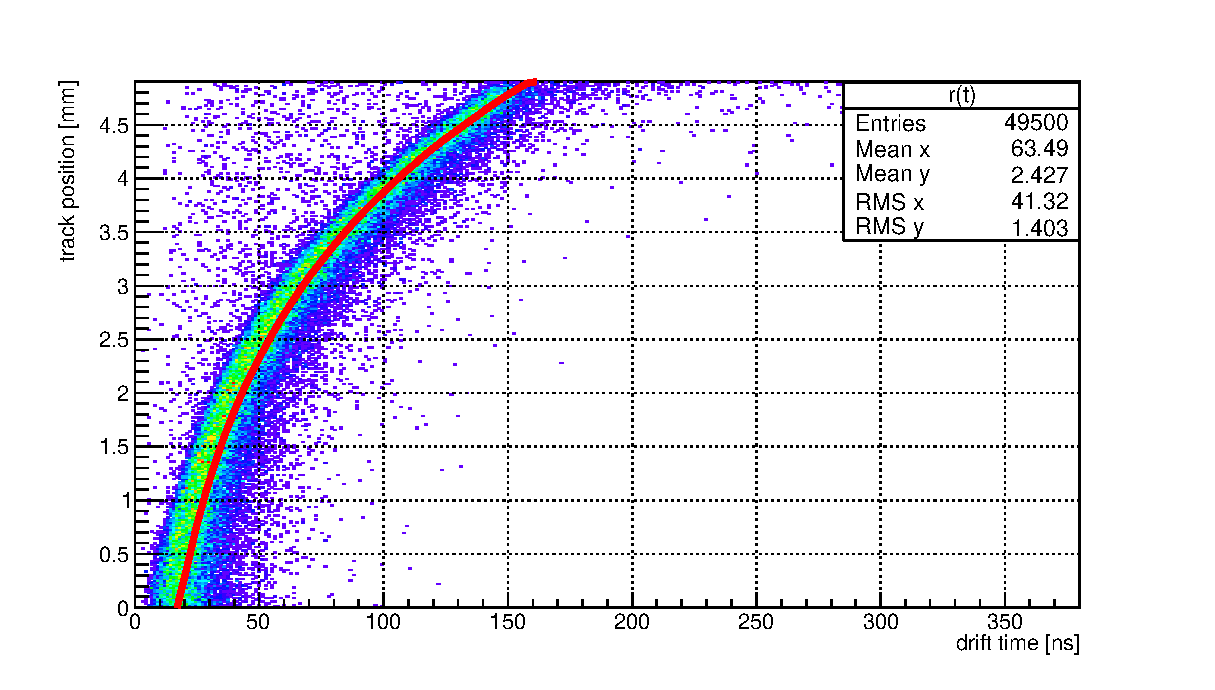
\includegraphics[width=0.7\textwidth]{rt_calibration.eps}
	\centering
	\caption{ RT-ralation(calibration line, figured in red color) between drift time $t_{drift}$ and distance from the  track $r_{track}$ .  The fit is performed in the range of
$0 < t_{drift} < 150 ns$ and $|r| < 4.9mm$ }
	\label{fig:calibration_00}
	\end{figure}
	
	Далі наводимо параметри калібровочної кривої як результат фітування розподілу $t_{drift}(r)$ Рис. \ref{fig:calibration_00} 
	
	\begin{itemize}
		\item $a_1 = 2.231 \pm 0.008$
		\item $a_2 = 0.448 \pm 0.002$
	\end{itemize}
	
	\subsubsection{Precision of track reconstruction}	

	\subsubsection{ How precision of track reconstruction depend on wire displacement }
	Для початку задамося питанням "як точність реконструкції треків залежить 	від положення дроту (точніше від його відхилення від центрального положення).
	
	Відомо, що робочі зразки дрейфових трубок будуть працювати в горизонтальному положенні. Зважаючи, що під дією гравітаційного поля дріт в трубці буде прогинатися вниз, можна з певною достовірністю стверджувати про подальше положення дроту, вже після підведення напруги в трубці.
	
	Так виконаємо оцінку залежності точності вимірювання координати в трубці  по зміні часового розподілу.
	
	
	\subsubsection{Evaluation of track reconstruction precision}
	Похибкою вимірювання положення треку будемо називати різницю між дійсним положенням треку $r_{track}$ and reconstructed $r_{rec}$. Дану точку відобразим на графіку з відхиленням по осі Y та дійсним положенням треку по осі X. Для більшої наглядності ситуації з розподілом точок на графіку зобразимо цю ж інформацію у вигляді діаграми густини точок а також у виляді труктурної діаграми для  оцінки абсолютної похибки.
	
	Варто зазначити, калібровочна крива не проходить через точку $(0;0)$, то ж значення часу дрейфу ліворуч від кривої будемо співставляти центральний трек (такий, що проходить через центр дрейфової трубки $r=0$). Схоже правило застосовується для сигналів з часом дрейфу більшим за діапазон охоплений калібровочною кривою - таким сигналам $r_{reconstructed}$ присвоюється значення $r_{tube} = 4.9mm$.
	
	\begin{figure}[h]
	\centering
		\subfloat[Distribution of  $r_{track} - r_{rec}$ value]{
			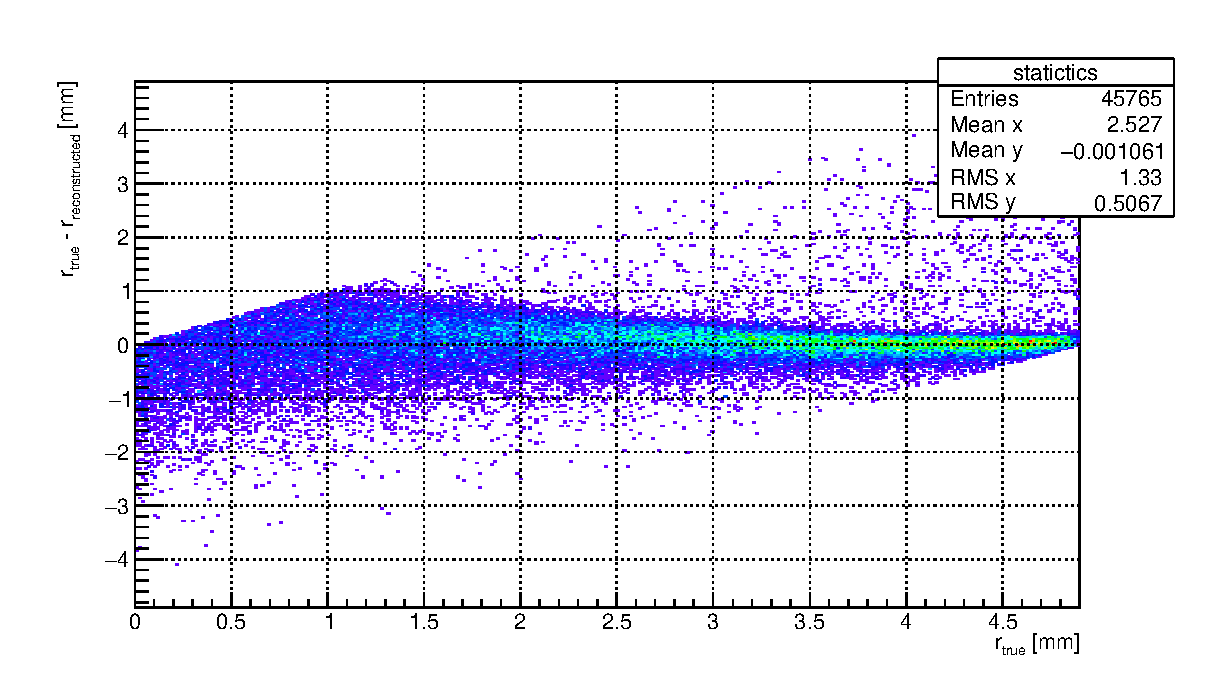
\includegraphics[width=0.45\textwidth]{difference_map_00.eps} 
			\label{fig:precision_00} }%
		\qquad
		\subfloat[projection of (a) along ]{
			\includegraphics[width=0.45\textwidth]{delta_structed.eps} 
			\label{fig:delta_sructed_00} }%
		\caption{Distribution of Розподіл різниці між дійсним і реконструйованим положенням треку в трубці $\bigtriangleup_{r_{track} - r_{rec}}$ від 49500 подій. Структурна діаграма розподілу точок у вападку строго центрального положення дроту дрейфової трубки}
	\end{figure}
	
	Як видно з простого аналізу діаграми Рис. \ref{fig:precision_00} \ref{fig:delta_sructed_00} точність реконструкції позиції треків лежить в діапазоні $(0.1 \dots 0.2) mm$. 
	
	\subsection{Випадок зміщеного дроту}
	Знаходження калібровочної кривої, якщо її так можна назвати, для випадку зміщеного дроту дещо відрізняється від описаного вище центрального випадку. Це пов’язано з несиметричністю розподілу ``час дрейфу - положення треку'' Рис. \ref{fig:tr_distr_15}. Тож необхідно знайте не одну, а дві калібровочні криві, причому необхідно розділення даних(на гілки більшу-меншу) що неможливо без попередньої оціки величини зміщення дроту від центрального положення.
	
	\begin{figure}
		\centering
		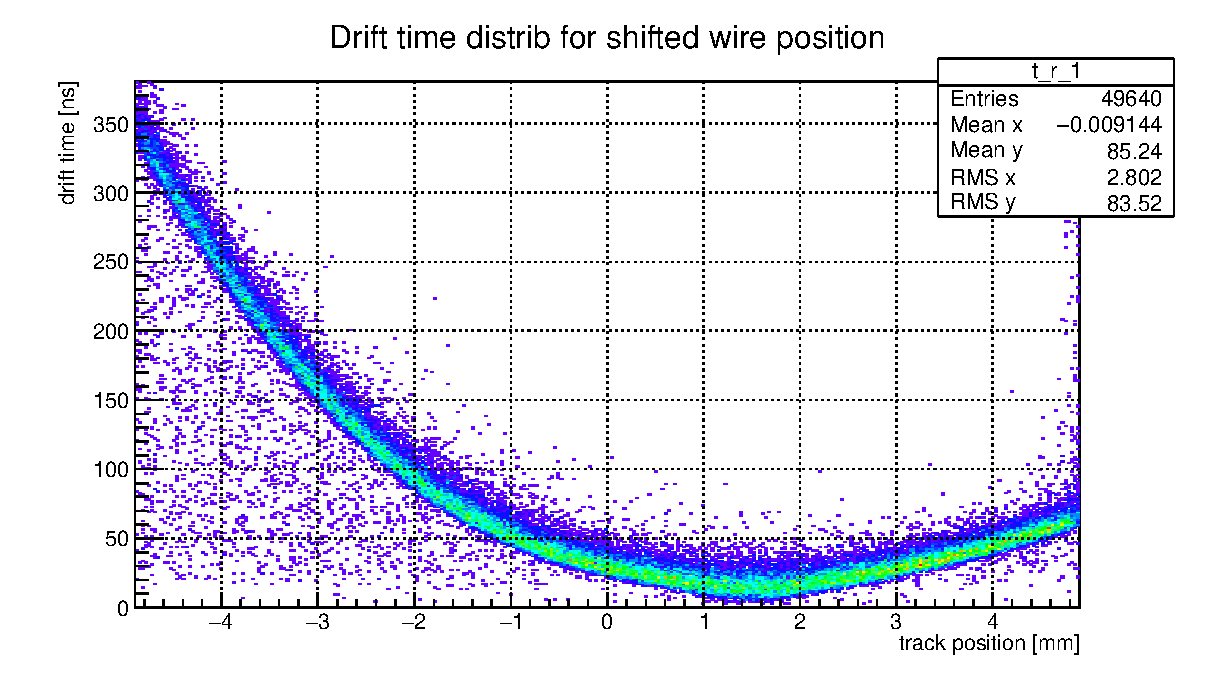
\includegraphics[width = \textwidth]{tr_distr_15.eps}
		\caption{TR-distribution for 1.5 mm shifted wire}
		\label{fig:tr_distr_15}
	\end{figure}
	
	Як видно з Рис \ref{fig:tr_distr_15} фігура розподілу змінилася не значно, а лише зсунулася на стале значення, рівне зміщенню дроту.
	
	Використаємо цю хитрість для розбиття даних на дві частини - дві гілки в RT розподілі. Від так ми можемо для  кожної гілки знайти свою власну калібровочну криву.
	
	\subsection{ Порівняння розподілів для центрального та зміщеного позицій дроту в трубці}	
	Наведемо порівнняння гістограм для центрального та зміщеного позицій дроту для вибірки треків в околі дроту та на відстані 2 мм від нього.
	
	\begin{figure}[h!]
	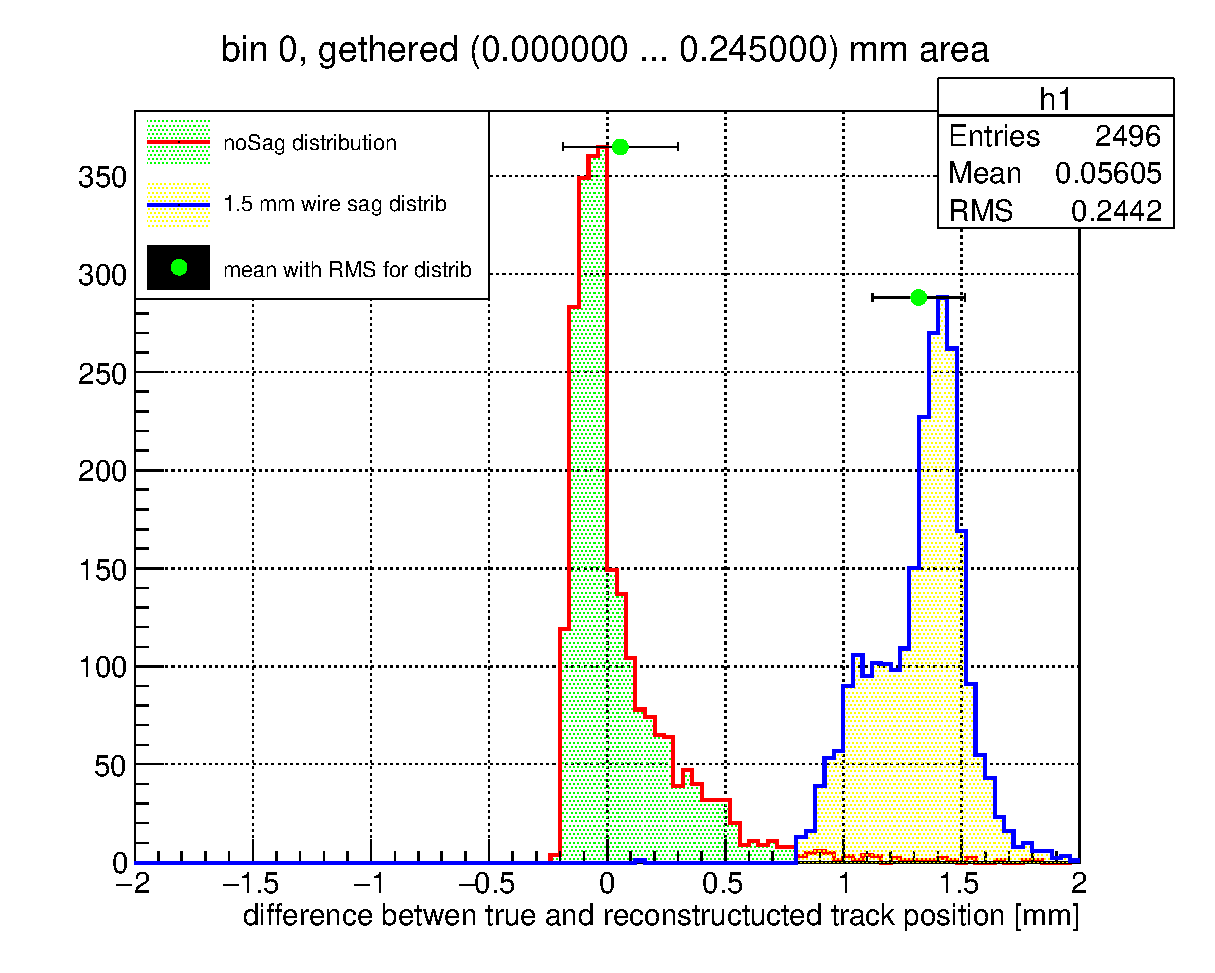
\includegraphics[width=0.8\textwidth]{bin0_0mm.eps}
	\centering
	\caption{ Порівняння розподілу реконструкції позицій треків для центрального положення дроту та вападку зміщення дроту дрейфової трубки на $1.5 mm$ від центрального положення для треків які проходять близько до центру трубки}
	\end{figure}
	
	\begin{figure}[h!]
	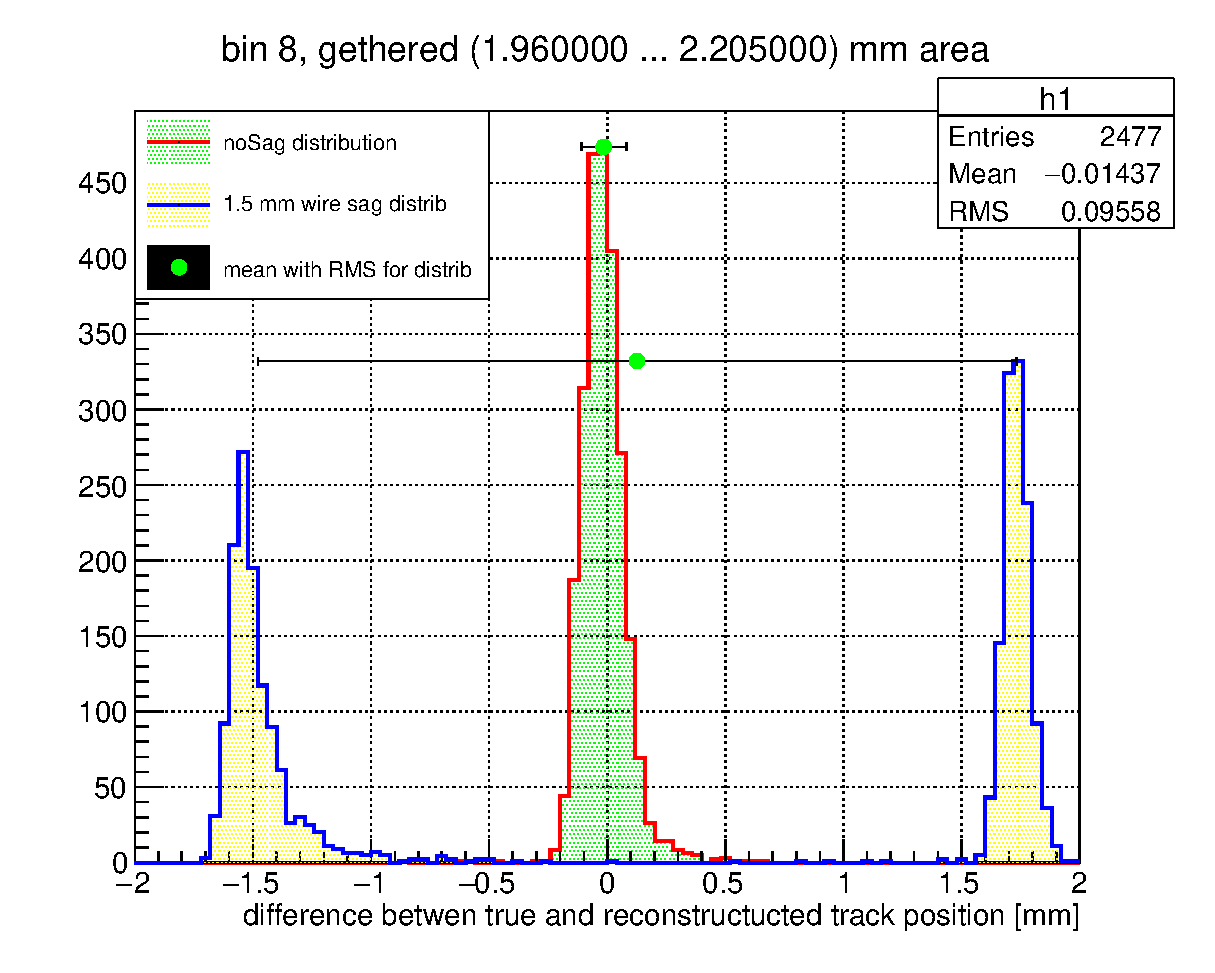
\includegraphics[width=0.8\textwidth]{bin8_2mm.eps}
	\centering
	\caption{ Порівняння розподілу реконструкції позицій треків для центрального положення дроту та вападку зміщення дроту дрейфової трубки на $1.5 mm$ від центрального положення для треків які проходять дотично до кола радусом $2mm$  коцентричного з трубкою}
	\end{figure}
	
	Цілком логічно припускати, що електроніка реєструватиме час дрейфу відмінний від триманого нами від симуляцій описаних вище. Тож необхідним буде врахувати внесок від електроніки. Ситуація ускладнюється тим що окрім форми вхідного сигналу потрібно знати ще й амплітуду сигналу(сумарний заряд зібраний з треку з урахуванням підсилення).
	
\newpage
\begin{thebibliography}{00}
	\bibitem{garfield} http://garfield.web.cern.ch/garfield

	\bibitem{kozlinskiy}  thesis Kozlinskiy.pdf 
	
\end{thebibliography}
	
\end{document}